\documentclass{article}
\usepackage[utf8]{inputenc}
\usepackage[english]{babel}
\usepackage{hyperref}

% graphics
\usepackage{graphicx}
\usepackage{float}
\graphicspath{{figures/}}

% todo notes
\usepackage{todonotes}
\let\oldtodo\todo
\renewcommand{\todo}[1]{\oldtodo[noline]{#1}}

% math stuff
\usepackage{amsmath}
\usepackage{amssymb}
\usepackage{amsthm}
\usepackage{commath}
\newcommand{\RR}{\mathbb{R}}
\newcommand{\NN}{\mathbb{N}}
\newcommand{\ZZ}{\mathbb{Z}}
\newcommand{\T}[1]{#1^{\top}}
\newcommand{\kth}[2][k]{#2^{(#1)}}
\newcommand{\Lip}[3]{\mathcal{F}_{#1}^{#2, #3}}
\newcommand{\Strong}[4]{\mathcal{S}_{#1, #2}^{#3, #4}}
\newcommand{\strong}[2]{\mathcal{S}_{#1}^{#2}}
\newcommand{\Lipl}{\Lip{L}{1}{1}}
\newcommand{\strongm}{\strong{\mu}{1}}
\newcommand{\Strongml}{\Strong{L}{\mu}{1}{1}}
\newcommand{\iprod}[2]{\left\langle #1, #2 \right\rangle}

\DeclareMathOperator{\diag}{diag}
\DeclareMathOperator*{\argmin}{arg min}
\DeclareMathOperator{\Span}{span}
\DeclareMathOperator{\proj}{proj}
\DeclareMathOperator{\card}{card}
\DeclareMathOperator{\tr}{tr}
\DeclareMathOperator{\rank}{rank}

\hyphenation{Lip-schitz}

% layout/sectioning
\newcounter{summary}[section]
\newcommand{\summary}[1]{%
  \paragraph{\arabic{section}.\arabic{summary}\enspace #1.}\refstepcounter{summary}}
\newcommand{\optionalsummary}[1]{%
  \paragraph{\arabic{section}.\arabic{summary}*\enspace #1.}\refstepcounter{summary}}
\renewcommand{\thesummary}{\thesection .\arabic{summary}}

\newtheoremstyle{slplain}% name
  {.5\baselineskip\@plus.2\baselineskip\@minus.2\baselineskip}% Space above
  {0pt}% Space below
  {\itshape}% Body font
  {}%Indent amount (empty = no indent, \parindent = para indent)
  {\bfseries}%  Thm head font
  {.}%       Punctuation after thm head
  { }%      Space after thm head: " " = normal interword space;
        %       \newline = linebreak
  {}%       Thm head spec
\theoremstyle{slplain}
\newtheorem{question}{Question}

\usepackage{parskip}



%%% Local Variables:
%%% mode: latex
%%% TeX-master: "summary"
%%% End:


% toc customization
\usepackage{tocloft}
\setcounter{tocdepth}{4}
\cftsetindents{paragraph}{0ex}{5ex}

\title{Summary of OCS Slides}
\author{Philipp Gabler}

\begin{document}
\maketitle

\tableofcontents
\newpage


%%%%%%%%%%%%%%%%%%%%%%%%%%%%%%%%%%%%%%%%%%%%%%%%%%%%%%%%%%%%%%%%%%
\noindent First of all, the \href{http://web.mit.edu/6.252/www/LectureNotes/}{material} by the
course of Dimitri P. Bertsekas cover pretty much the same as this. What a coincidence.

Secondly, sections marked with a star are additional material that is maybe useful, but was not
covered completely (or at all) in this course.  It is mainly taken from the more theoretical course
on convex optimization.

\section{Mathematical Preliminaries}


\summary{Basic Math}\label{s:basics}

Always remember these:
\begin{gather*}
  \nabla_x \frac{1}{2} \T{x}Qx + \T{c}x = Qx + c, \\
  \nabla_x \frac{1}{2} \enVert[1]{Ax - b} = \T{A}(Ax - b).
\end{gather*}
Futhermore, it is useful to know that
\begin{equation*}
  A = \begin{pmatrix}
    a & b \\
    c & d
  \end{pmatrix} \Rightarrow A^{-1} = \frac{1}{\det A}
  \begin{pmatrix}
    d & -b \\
    -c & a
  \end{pmatrix},
\end{equation*}
for
\begin{equation*}
  \det A = ad - cb \neq 0,
\end{equation*}
as well as the Taylor expansion around \(x_0\):
\begin{equation*}
  f(x) = f(x_0) + \T{\nabla f(x_0)}(x - x_0) + \frac{1}{2} \T{(x - x_0)}\nabla^2 f(x_0)(x - x_0)
  + o(\,\enVert{x - x_0}^2).
\end{equation*}


\summary{Calclulating Eigenvalues by Hand}
% calclulating eigenvalues by hand:
% http://math.harvard.edu/archive/21b_fall_04/exhibits/2dmatrices/index.html
% https://math.stackexchange.com/questions/395698/fast-way-to-calculate-eigen-of-2x2-matrix-using-a-formula

Given
\begin{equation*}
  A = \begin{pmatrix}
    a & b \\
    c & d\\
  \end{pmatrix},
\end{equation*}
we have \(\tr(A) = a + d\).  Then the characteristic polynomial can be written as
\begin{equation*}
  \lambda^2 - \lambda \tr(A) + \det(A) = 0.
\end{equation*}
This can be solved in the usual way by using the quadratic solution formula or by factorization.

The corresponding eigenvectors can then be written as follows:
\begin{itemize}
\item If \(c \neq 0\), they are
  \begin{equation*}
    \begin{pmatrix}
      \lambda_1 - d \\
      c 
    \end{pmatrix},
    \begin{pmatrix}
      \lambda_2 - d \\
      c 
    \end{pmatrix}.
  \end{equation*}.
\item If \(b \neq 0\), they are
  \begin{equation*}
    \begin{pmatrix}
      b \\
      \lambda_1 - a
    \end{pmatrix},
    \begin{pmatrix}
      b \\
      \lambda_2 - a 
    \end{pmatrix}.
  \end{equation*}
\item If \(b = c = 0\), they are
  \begin{equation*}
    \begin{pmatrix}
      1 \\
      0
    \end{pmatrix},
    \begin{pmatrix}
      0 \\
      1
    \end{pmatrix}.
  \end{equation*}
\end{itemize}


\summary{Definiteness}\label{s:definiteness}

A symmetric matrix \(Q\) is called \emph{positive semidefinite} if \(\T{x} Q x \geq 0\) for all
\(x\), and \emph{positive definite} if \(\T{x} Q x > 0\) for all \(x \neq 0\).  Sometimes this is
written as \(Q \succeq 0\) and
\(Q \succ 0\).\footnote{\url{https://en.wikipedia.org/wiki/Positive-definite_matrix}} In the case of
\(Q \in \RR^{2 \times 2}\), we can use the following criteria:
\begin{enumerate}
\item \(Q \succeq 0 \Leftrightarrow \det Q \geq 0, Q_{11} \geq 0, Q_{22} \geq 0\) 
\item \(Q \succ 0 \Leftrightarrow \det Q > 0, Q_{11} > 0 \Leftrightarrow \) all eigenvalues of \(Q\)
  are positive.
\end{enumerate}

The notation can also be used for general inequalities between quadratic forms: \(a \preceq Q
\preceq b \Leftrightarrow \forall x: a \leq \T{x}Qx \leq b\), etc.

\optionalsummary{Norms}\label{s:norms}

As usual, we have the \(\ell_p\)-norms for \(x \in \RR^N\):
\begin{equation*}
  \lVert x \rVert_p = \left( \sum_{1 \leq i \leq N} |x_i|^p \right).
\end{equation*}

Special cases of this are the \emph{Euclidean norm} (\(p = 2\)) and the \emph{Manhatton norm}
(\(p = 1\)):
\begin{equation*}
  \lVert x \lVert_2 = \sqrt{\T{x} x} \quad \text{and} \quad \lVert x \lVert_1 = \sum_{1 \leq i \leq
    N} |x_i|.
\end{equation*}
The Manhattan norm is used mostly in regularization terms to achieve sparse values.  In the limit,
there are the \(\ell_\infty\)- or \emph{maximum norm} and the \(\ell_0\)-quasinorm:
\begin{equation*}
  \lVert x \lVert_\infty = \max_i \{|x_i|\} \quad
\text{and} \quad \lVert x \lVert_0 = \card \{i \mid x_i \neq 0\}.
\end{equation*}
The \(\ell_0\)-norm counts the number of nonzero entries in a vector, and is the strongest possible
sparsity constraint.  It usually is replaced by the \(\ell_1\)-norm in practical applications.

For matrices in \(\RR^{m \times n}\), we can consider so-called \emph{operator norms}.  An operator
\(A: X \to Y\) between normed spaces is called bounded by a number \(C\) if for all \(x \in X\)
\begin{equation*}
  \lVert Ax \rVert_Y \leq C \lVert x \rVert_X.
\end{equation*}
The operator norm is the smallest bound of it:
\begin{equation*}
  \lVert A \rVert_{X,Y} = \sup_x \frac{\lVert Ax \rVert_Y}{\lVert x \rVert_X}
  = \sup_{\lVert x \rVert_X \leq 1} \lVert Ax \rVert_Y.
\end{equation*}
If \(A\) can be described by a matrix, we can use \(p\)-norms again and write \(\lVert A
\rVert_{p,q}\).

Based on the operator norm, we can form the \emph{dual norm} of a norm \(\lVert \cdot \rVert\):
\begin{equation*}
  \lVert y \rVert_{*} = \sup_{\lVert x \rVert \leq 1} \T{y} x,
\end{equation*}
which is the operator norm of \(y\) when treated as a dual vector.  If \(\lVert \cdot \rVert\) is an
\(\ell_p\)-norm, then the dual is the \(\ell_q\)-norm with \(\frac{1}{q} + \frac{1}{p} = 1\).

A further family of matrix norms are the \emph{Schatten \(p\)-norms}.  For a matrix \(A \in
\RR^{M \times N}\) with rank \(R\), consider the singular value decomposition
\begin{equation*}
  A = U \Sigma \T{V},
\end{equation*}
where \(U \in \RR^{M \times R}\), \(V \in \RR^{R \times N}\) are orthogonal and
\(\Sigma = \diag(\sigma_1, \ldots, \sigma_R) \in \RR^{R \times R}\).  It holds that
\(\sigma_i(A) = \sqrt{\lambda_i(A \T{A})}\).  Then we can define norms
\begin{equation*}
  \lVert A \rVert_{S_p} = \left( \sum_{1 \leq i \leq R} \sigma_i(A)^p \right).
\end{equation*}
These norms are based solely on the eigenvalues; they measure the stretching of the matrix
(described by \(\Sigma\)), while ignoring the rotation part.  Special cases here are the
\emph{nuclear norm} (\(p = 1\))
\begin{equation*}
  \lVert A \rVert_{*} = \sum_{1 \leq i \leq R} \sigma_i(A),
\end{equation*}
the \emph{Frobenius norm} (\(p = 2\))
\begin{equation*}
  \lVert A \rVert_{F} = \sqrt{\sum_{1 \leq i \leq R} \sigma_i^2(A)}
    = \sqrt{\tr(A\T{A})} = \sqrt{\sum_{ij} a_{ij}^2}
\end{equation*}
as well as the limit cases of the \emph{spectral norm} and the rank:
\begin{equation*}
  \lVert A \rVert_{\infty} = \max\{\sigma_1, \ldots, \sigma_R\} \quad \text{and} \quad
  \lVert A \rVert_{0} = R = \rank(A).
\end{equation*}

\summary{Convex Sets}\label{s:convex_sets}

A set \(X\) is convex, if for all \(x, y \in X\) and \(\alpha \in [0,1]\):
\begin{equation*}
  \alpha x + (1 - \alpha) y \in X.
\end{equation*}
This means that \(X\) contains all convex combinations of points from it.

If \(C_1\) and \(C_2\) are convex sets, then also \(C_1 \cap C_2\) and \(C_1 + C_2\) (Minkowski sum)
are.  Examples of convex sets are convex hulls, planes, halfspaces, polyhedra, norm balls, and
cones. 

\summary{Level Sets}\label{s:level-sets}

For a function \(f: X \to \RR\), and \(c \in \RR\), the sets
\begin{equation*}
  S_c(f) = \{x \in X: f(x) = c\}
\end{equation*}
are called \emph{level sets} of \(f\). They can be convex even if \(f\) is not!

\summary{Convex Functions}\label{s:convex_functions}

If \(X\) is a convex set in some vector space, then \(f: X \to \RR\) is called \emph{convex} if for
all \(x, y \in X\) and \(\alpha \in [0,1]\):
\begin{equation*}
  f(\alpha x + (1 - \alpha) y) \leq \alpha f(x) + (1 - \alpha) f(y).
\end{equation*}
This means that no points lie below any tangent.  Equivalent to this, for sufficiently
differentiable functions, are the first-order condition
\begin{equation*}
  f(x) \geq f(y) + \T{\nabla f(y)}(x - y), \quad \forall x, y \in X
\end{equation*}
and the second-order condition
\begin{equation*}
  \nabla^2 f(x) \succeq 0 \quad \forall x \in X.
\end{equation*}
We speak about \emph{strict convexity} when the inequalities are replaced by strict ones.

\summary{Strong Convexity}\label{s:strong-convexity}

A function \(f: X \to \RR\) is \emph{\(\mu\)-strongly
  convex}\footnote{\url{https://en.wikipedia.org/wiki/Convex_function\#Strongly_convex_functions}}
(for \(\mu > 0\)) if for all \(x, y \in X\) and \(\alpha \in [0,1]\):
\begin{equation*}
  f(\alpha x + (1 - \alpha) y) \leq \alpha f(x) + (1 - \alpha) f(y)
  - \frac{\mu}{2} \alpha (1 - \alpha) \enVert[1]{x - y}^2,
\end{equation*}
or equivalently for differentiable functions:
\begin{equation*}
  f(x) \geq f(y) + \T{\nabla f(y)}(y - x) + \frac{\mu}{2}\enVert[1]{y - x}^2
  \quad \forall x, y \in X,
\end{equation*}
and twice differentiable functions:
\begin{equation*}
  \nabla^2 f(x) \succeq \mu \quad \forall x \in X.
\end{equation*}
The latter is equivalent to requiring that the minimum eigenvalue of \(\nabla^2 f(x)\) is at least
\(\mu\) for all \(x\).  This definition approaches the definition for strict convexity as
\(\mu \to 0\), and is identical to the definition of a convex function when \(\mu = 0\).  On
\(X = \RR\), \(f\) is \(\mu\)-strongly convex if \(f''(x) \geq \mu > 0\) for all \(x\).

\begin{figure}[H]
  \centering
  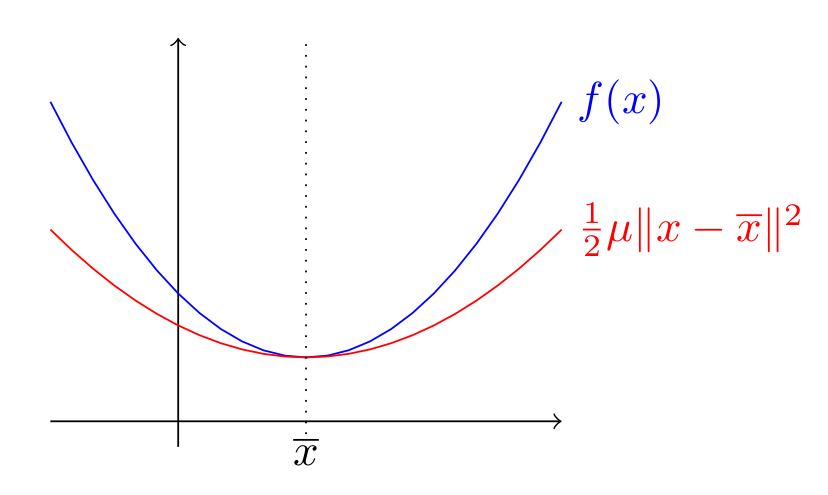
\includegraphics[width=0.5\textwidth]{strong_convexity}
  \caption{Illustration of the lower bound provided by strong
    convexity.\label{fig:strong-convexity}}
\end{figure}

Strong convexity means that the function can be bounded from below by a quadratic function: if
\(\nabla f(x^*) = 0\), then
\begin{equation*}
  f(x) \geq f(x^*) + \frac{\mu}{2} \enVert{x - x^*}^2;
\end{equation*}
see Figure~\ref{fig:strong-convexity}.


\summary{Lipschitz continuity}\label{s:lipschitz-continuity}

A function \(f: \RR^n \to \RR\) is called \emph{Lipschitz continuous}, if there is value
\(L \geq 0\), called \emph{Lipschitz constant}, such that for all \(x, y \in \RR^n\)
\begin{equation*}
  \enVert{f(x) - f(y)} \leq L \enVert[1]{x - y}.
\end{equation*}
for some norm.  This is equivalent to
\begin{equation*}
  \enVert{f(x + ty) - f(x)} \leq Lt \enVert[1]{y} \quad \forall t \in [0, 1].
\end{equation*}

Lipschitz continuity implies continuity.

Intuitively, a Lipschitz continuous function is limited in how fast it can change: there exists a
Lipschitz constant such that, for every pair of points on the graph of this function, the absolute
value of the slope of the line connecting them is not greater than this
constant.\footnote{\url{https://en.wikipedia.org/wiki/Lipschitz_continuity}}

A differentiable function \(\RR \to \RR\) is Lipschitz continuous with \(L = \sup_x |g'(x)|\) if
and only if it has a bounded first derivative.

\optionalsummary{Lipschitz-continuous gradients and strong convexity}
\label{s:lipschitz-strong-convexity}

Let us denote the following classes of \emph{covex} functions:
\begin{itemize}
\item \(\Lip{L}{n}{k}\): \(n\) times continuously differentiable convex functions with
  \(L\)-Lipschitz continuous \(k\)-th derivative,
\item \(\strong{\mu}{n}\): \(n\) times continuously differentiable \(\mu\)-strongly
convex functions, and
\item \(\Strong{L}{\mu}{n}{k}\): \(n\) times continuously differentiable
  \(\mu\)-strongly convex functions with \(L\)-Lipschitz continuous \(k\)-th derivative.
\end{itemize}
(Where \(\Strong{L}{0}{n}{k} = \Lip{L}{n}{k}\), obviously.)

First, there is a genenal second-order characterization for \(f \in \Strong{\mu}{L}{2}{1}\):
\begin{equation*}
  \mu \preceq \nabla^2 f(x) \preceq L.
\end{equation*}

Then, we have a range of properties of the classes of convex functions with Lipschitz-continuous
gradient and of \(\mu\)-strongly convex differentiable functions, which are the ones we usually deal
with in first-order gradient methods. There are a couple of remarkable symmetries between properties
of them, listed below; in each case except the last, the whole statement holds for
\(f \in \Strong{\mu}{L}{1}{1}\), but both sides hold individually in \(\smash{\strongm}\) and
\(\smash{\Lipl}\), respectively.

\begin{enumerate}
\item The descent lemma (Summary~\ref{s:descent-lemma}) and its converse, which bound the first
  order approximation around a point:
  \begin{align*}
    f(y) &\leq f(x) + \iprod{\nabla f(x)}{y - x} + \frac{L}{2}\enVert{y - x}^2 \\
    f(y) &\geq f(x) + \iprod{\nabla f(x)}{y - x} + \frac{\mu}{2}\enVert{y - x}^2 \\
  \end{align*}
  \vspace{-3em}
\item Their ``inverses'', bounding the first order approximation by the gradients:
  \begin{align*}
    f(y) &\geq f(x) + \iprod{\nabla f(x)}{y - x} + \frac{1}{2L}\enVert{\nabla f(x) - \nabla f(y)}^2 \\
    f(y) &\leq f(x) + \iprod{\nabla f(x)}{y - x} + \frac{1}{2\mu}\enVert{\nabla f(x) - \nabla f(y)}^2
  \end{align*}
\item A bound on the difference between gradients by values(the left inequality on the bottom is
  known as \emph{co-coercivity}):
  \begin{align*}
    \mu \enVert{x - y}^2 \leq \iprod{\nabla f(x) - \nabla f(y)}{x - y} &\leq L \enVert{x - y}^2 \\
    \frac{1}{L} \enVert{\nabla f(x) - \nabla f(y)}^2 \leq \iprod{\nabla f(x) - \nabla f(y)}{x - y}
    &\leq  \frac{1}{\mu} \enVert{\nabla f(x) - \nabla f(y)}^2 \\
  \end{align*}
  \vspace{-3em}
\item Finally, we have a combination of bounds with \(L\) and \(\mu\):
  \begin{equation*}
    \iprod{\nabla f(x) - \nabla f(y)}{x - y} \geq \frac{\mu L}{\mu + L}\enVert{x - y}^2 +
    \frac{1}{\mu + L} \enVert{\nabla f(x) - \nabla f(y)}^2
  \end{equation*}
\end{enumerate}

%%%%%%%%%%%%%%%%%%%%%%%%%%%%%%%%%%%%%%%%%%%%%%%%%%%%%%%%%%%%%%%%%%
\section{Introduction to Optimization}

\summary{General Form of Optimization Problems}\label{s:optimization-form}

A general minimization problem has the form
\begin{equation*}
  \min_{x} f(x) \quad \text{s.t. } x \in X,
\end{equation*}
for a \emph{constraint set} \(X \subseteq \RR^n\) (often given by some \emph{constraint functions})
and an \emph{objective function} \(f: X \to \RR\).  We want to find an optimal value or
\emph{minimizer} \(x^* \in X\) such that
\begin{equation*}
  f(x^*) \leq f(x), \quad \forall x \in X.
\end{equation*}


\summary{Types of Optimization Problems}\label{s:optimization-types}

\begin{enumerate}
\item
  \begin{enumerate}
  \item Discrete: \(X\) is a discrete set, also called \emph{integer programming}.
  \item Continuous: \(X\) is continuous (ie. uncountable)
  \end{enumerate}
\item
  \begin{enumerate}
  \item Linear: Objective functions and constraints are all linear:
    \begin{equation*}
      \min_x \T{c} x, \quad\text{s.t. } Ax \leq b,\; x \geq 0.
    \end{equation*}
    The constraints describe a convex polyhedron.  Polynomially solvable.
  \item Quadratic: Objective function is quadratic, constraints linear:
    \begin{equation*}
      \min_x \frac{1}{2}\T{x} Q x + \T{c} x, \quad\text{s.t. } Ax \leq b,\; Ex = d.
    \end{equation*}
    If \(Q\) is positive semidefinite, the objective is convex and the problem is polynomially
    solvable.
  \item Convex: objective function \(f\) and constraint set \(X\) are convex:
    \begin{equation*}
      \min_x f(x), \quad\text{s.t. } x \in X.
    \end{equation*}
    \vspace{-1.5em}
  \item Nonlinear: Nonlinear: no further requirements~-- objective function and constraints may be
    arbitrary.  Usually used if not known whether the problem is convex.  Not much theory available
    in general form.
  \end{enumerate}
\item
  \begin{enumerate}
  \item Unconstrained: Optimal solution searched in full \(\RR^n\). Easier to characterize, and
    usually to solve.
  \item Constrained: Optimal solution in an admissible region, usually more difficult to
    setup/characterize.
  \end{enumerate}
\end{enumerate}


\summary{Local and Global Minima}\label{s:local-global-minima}

A point \(x^*\) is called an \emph{unconstrained global minimum} of \(f\) if for all \(x\)
\begin{equation*}
  f(x^*) \leq f(x).
\end{equation*}
\(x^*\) is called an \emph{unconstrained local minimum} of \(f\) if it is minimal in some
neighbourhood; i.e., there is an \(\epsilon > 0\) such that
\begin{equation*}
  f(x^*) \leq f(x) \quad \forall x \text{ with } \lVert x^* - x \rVert \leq \epsilon.
\end{equation*}
For \emph{constrained} minima, we just require additionally that \(x^* \in X \subset \RR^n\).


\summary{First Order Neccessary Condition for Optimality}\label{s:first-order-optimality}

If \(f\) is continuously differentiable, then in a small neighbourhood of \(x^*\), we can by Taylor
expansion write \(f\) as
\begin{equation*}
  f(x) = f(x^* + \Delta x) = f(x^*) + \T{\nabla f(x^*)} \Delta x + o(\lVert \Delta x \rVert).
\end{equation*}
Since \(x^*\) is a local minimum, \(f(x^* + \Delta x) - f(x^*) \geq 0\), and we have
\begin{align*}
  0 &\leq f(x^* + \Delta x) - f(x^*) \\
    &\leq f(x^*) + \T{\nabla f(x^*)} \Delta x - f(x^*) \\
    &= \T{\nabla f(x^*)} \Delta x.
\end{align*}
Since we can equally choose \(\Delta x\) to have the opposite sign, we can do the same proof using
\(f(x^* - \Delta x)\), which results in
\begin{equation*}
  \T{\nabla f(x^*)} \Delta x \leq 0.
\end{equation*}
Combining both inequalities implies \(\T{\nabla f(x^*)} \Delta x = 0\).  Since \(\Delta x\) is
arbitrary, that implies that \(\nabla f(x^*) = 0\), which is the neccessary condition.  A point
which has this property is called a \emph{stationary point}.  In ``normal'' cases, it is either a
local optimum or a saddle point.


\summary{Second Order Neccessary Condition for Optimality}\label{s:second-order-optimality}

If \(f\) is twice continuously differentiable, then by second order Taylor expansion, we get
\begin{align*}
  0 &\leq f(x^* + \Delta x) - f(x^*) \\
    &= f(x^*) + \underbrace{\T{\nabla f(x^*)} \Delta x}_{=\; 0} +
      \frac{1}{2} \T{\Delta x} \nabla^2 f(x^*) \Delta x + o(\lVert \Delta x \rVert^2) - f(x^*) \\
    &=  \frac{1}{2} \T{\Delta x} \nabla^2 f(x^*) \Delta x + o(\lVert \Delta x \rVert^2).
\end{align*}
From this follows that \(\T{\Delta x} \nabla^2 f(x^*) \Delta x \geq 0\).  Since \(\Delta x\) is
arbitrary, this means that \(\nabla^2 f(x^*)\) must be positive semidefinite.  The interpretation of
this is that the function must be convex in some neighbourhood for for a point to be ``at least as
good as its neighbours''; if it is strictly convex, we get the following:


\summary{Sufficient Condition for Optimality}\label{s:sufficient-optimality}

If for a point \(x^*\) we have
\begin{equation*}
  \nabla f(x^*) = 0 \text{ and } \nabla^2 f(x^*) \succ 0,
\end{equation*}
(no ``semi-''!), then \(x^*\) is a strict unconstrained local minimum of \(f\).  (The reason for
this is that in this case, \(f\) is locally strictly convex, and thus a stationary point is
neccessaryly an optimum.)


\summary{Minima of Convex Functions}\label{s:convex-minima}

For a convex function \(f\), local minima are also global minima: suppose \(x^*\) were a local, but
not global minimum.  Then there must be some \(y^* \neq x^*\) with \(f(y^*) < f(x^*)\).  But by
convexity, we have for all \(\alpha \in [0, 1)\):
\begin{equation*}
  f(\alpha x^* + (1 - \alpha) y^*) < \alpha f(x^*) + (1 - \alpha) f(y^*) < f(x^*),
\end{equation*}
which contradicts the assumption of \(x^*\) being minimal in a local environment. Therefore \(x^*\)
must also be a global minimum.

Furthermore, the neccessary condition for minima, \(\nabla f(x^*) = 0\), for convex functions
becomes a sufficient condition: assume \(\nabla f(x^*) = 0\), but \(x^*\) were not optimal, so there
is a \(y^*\) with \(f(y^*) < f(x^*)\).  Then, by the first order convexity condition of \(f\) (see
Summary~\ref{s:convex_functions}),
\begin{align*}
  f(y^*) &\geq f(x^*) + \underbrace{\T{\nabla f(x^*)}}_{=\, 0}(y^* - x^*) \\
         &= f(x^*);
\end{align*}
this contradicts the assumption, therefore \(x^*\) must be optimal.

\optionalsummary{Existence of Minimizers}\label{s:minimizers-existence}

A crucial condition for the general existence of minimizers is the following: a function
\(f: X \subset \RR^N \to \RR \cup \{\infty\}\) is \emph{lower semicontinuous (lsc)}, if for all
sequences \({x_k} \in X\) converging to \(x \in X\) we have that
\begin{equation*}
  f(x) \leq \liminf_{k \to \infty} f(x_k).
\end{equation*}
If \(f\) is such, we can prove by the Heine-Borel theorem that if \(X\) is closed and bounded, \(f\)
has a global minimizer.

If \(X\) is not bounded, we cannot use a compactness argument, but need an additional condition:
\(f\) is called \emph{coercive} if for every sequence \({x_k} \in X\) with \(\lVert x_k \rVert \to
\infty\), \(f(x_k) \to \infty\).  Now, if \(f\) is lower semicontinuous and coercive, and \(X\) is
closed and non-empty, then \(f\) also has a global minimizer.

%%%%%%%%%%%%%%%%%%%%%%%%%%%%%%%%%%%%%%%%%%%%%%%%%%%%%%%%%%%%%%%%%%
\section{Gradient Methods}

\summary{Basic Idea}\label{s:gradient-methods}

To find a minimum of \(f\), we construct a sequence \(\kth{x}\) such that for all \(k\),
\(f(\kth[k+1]{x}) < f(\kth{x})\).  To do that, we choose an initial \(\kth[0]{x}\) and then set
\begin{equation*}
  \kth[k+1]{x} = \kth{x} + \kth{\alpha} \kth{d}.
\end{equation*}
Here \(\kth{\alpha}\) is some step size, and \(\kth{d}\) is a \emph{descent direction} which must
satisfy
\begin{equation*}
  \pd{f}{{\kth{d}}}(\kth{x}) = \T{\nabla f(\kth{x})} \kth{d} < 0, 
\end{equation*}
where \(\pd{f}{{\kth{d}}}\) is the directional derivative in direction \(\kth{d}\).


\summary{Matrix-Scaled Gradients}\label{s:scaled-gradients}

Given the above form, one can choose \(\kth{d} = -\kth{D} \nabla f(\kth{x})\) for a positive
definite \(\kth{D}\).  That this gives a descent direction follows directly from positive
definiteness:
\begin{equation*}
  \T{\nabla f(\kth{x})} \kth{d} = -\T{\nabla f(\kth{x})} \kth{D} \nabla f(\kth{x}) < 0,
\end{equation*}
(since \(\T{x}\kth{D}x > 0\) for all \(x\)).

\begin{enumerate}
\item Steepest descent: \(\kth{D} = I\).  Slow convergence if the level lines are elongated (leads
  to zig-zagging), but easy to evaluate.
\item Newton's method: \(\kth{D} = (\nabla^2 f(\kth{x}))^{-1}\).  Very fast convergence near minima,
  but unstable wrt. initial values (may diverge).  Requires recalculation of inverse of Hessian in
  every step~-- very expensive in large dimensions.  \(\nabla^2 f(\kth{x})\) might become singular.
  Corresponds to local approximation by a quadratic surface (see
  Summary~\ref{s:newton-method-derivation}).
\item Levenberg-Marquart method: \(\kth{D} = (\nabla^2 f(\kth{x}) + \lambda I)^{-1}\).  Tries
  to fix problems with Newton's method by regularization (see Summary~\ref{s:levenberg-method}).
\item Diagonal scaling: \(\kth{D} = \diag(\kth{d}_1, \ldots, \kth{d}_n)\). E.g. approximating
  Newton's method with
  \begin{equation*}
    \kth{d}_i = \left( \pd[2]{f}{x_i}(\kth{x}) \right)^{-1},
  \end{equation*}
  but usually not worth it (scales only in diagonal directions).
\item Gauss-Newton method: For a nonlinear least-squares problem
  \(f(x) = \frac{1}{2} \lVert g(x) \rVert^2\), we can choose
  \(\kth{D} = ( \nabla g(\kth{x}) \T{\nabla g(\kth{x})} )^{-1}\).  This is related to the
  pseudo-inverse (see Summary~\ref{s:gauss-newton-method}).
\end{enumerate}


\summary{Step Size Selection}\label{s:step-size-selection}

To ensure convergence and performance, \(\kth{\alpha}\) needs to be chosen with care.
Theoretically, it is not enough set it such that \(f(\kth[k+1]{x}) < f(\kth{x})\); there are
counterexamples for which this holds, but we have \(\lim_{k \to \infty} f(\kth{x}) > f(x^*)\), e.g.,
when the step sequence in the limit oscillates between two values on the opposite sides of a
``bowl'' (cf. Summary~\ref{s:gradient-related-condition}).

Some usual approaches to choosing the step size are:
\begin{enumerate}
\item Minimization rule: choose \(\kth{\alpha}\) such that the minimum in the descent direction is
  taken, i.e.
  \begin{equation*}
    f(\kth{x} + \kth{\alpha}\kth{d}) = \min_{\alpha \geq 0} f(\kth{x} + \alpha\kth{d}).
  \end{equation*}
\item Limited minimization rule: ``heuristically'' search the best \(\kth{\alpha}\) in some set,
  like in an interval \([0, s]\) or among some values \(\{\beta^0 s, \beta^1 s, \ldots \}\) for some
  fixed \(\beta \in (0, 1)\) and \(s > 0\).
\item Constant step size: sometimes, an optimal (or good enough) value \(\kth{\alpha} = s\) can be
  computed from the objective function in advance.
\item Diminishing step size: choose a decreasing sequence with
  \(\lim_{k \to \infty} \kth{\alpha} = 0\) and \(\sum_{k = 0}^{\infty} \kth{\alpha} = \infty\).  The
  latter is sufficient to ensure convergence (we can never ``run out of space'' before the optimum
  is reached).  This has good theoretical properties for some setups, but the convergence rate can
  be quite slow.
\end{enumerate}


\summary{Armijo Rule}\label{s:armijo-rule}

This is a special method for step size selection, which has nice theoretical properties (e.g. using
it, the \(\kth{x}\) always converge to a stationary point).  To apply it, we fix an initial step
size \(s\), a reduction factor \(0 < \beta < 1\), and a scalar \(0 < \sigma < 1\), and choose
\(\kth{m}\) as the first nonnegative integer for which
\begin{equation*}
  f(\kth{x} + \beta^{\kth{m}} s \kth{d}) - f(\kth{x}) \leq
  \sigma \beta^{\kth{m}} s \nabla \T{f(\kth{x})} \kth{d}.
\end{equation*}
Then, set \(\kth{\alpha} = \beta^{\kth{m}} s\).  (Usually, \(\sigma \in [10^{-5}, 10^{-1}]\),
\(\beta \in [1/10, 1/2]\), and \(s = 1\).)

The interpretation of this is that we use \(1, \beta, \beta^2, \ldots\) succesively, to try out the
step sizes \(\beta^{\kth{m}} s\) in decreasing order, until we find one for which the decrease in
the objective is sufficiently large for \(\kth{m}\) (see Figure~\ref{fig:armijo}).

\begin{figure}[H]
  \centering
  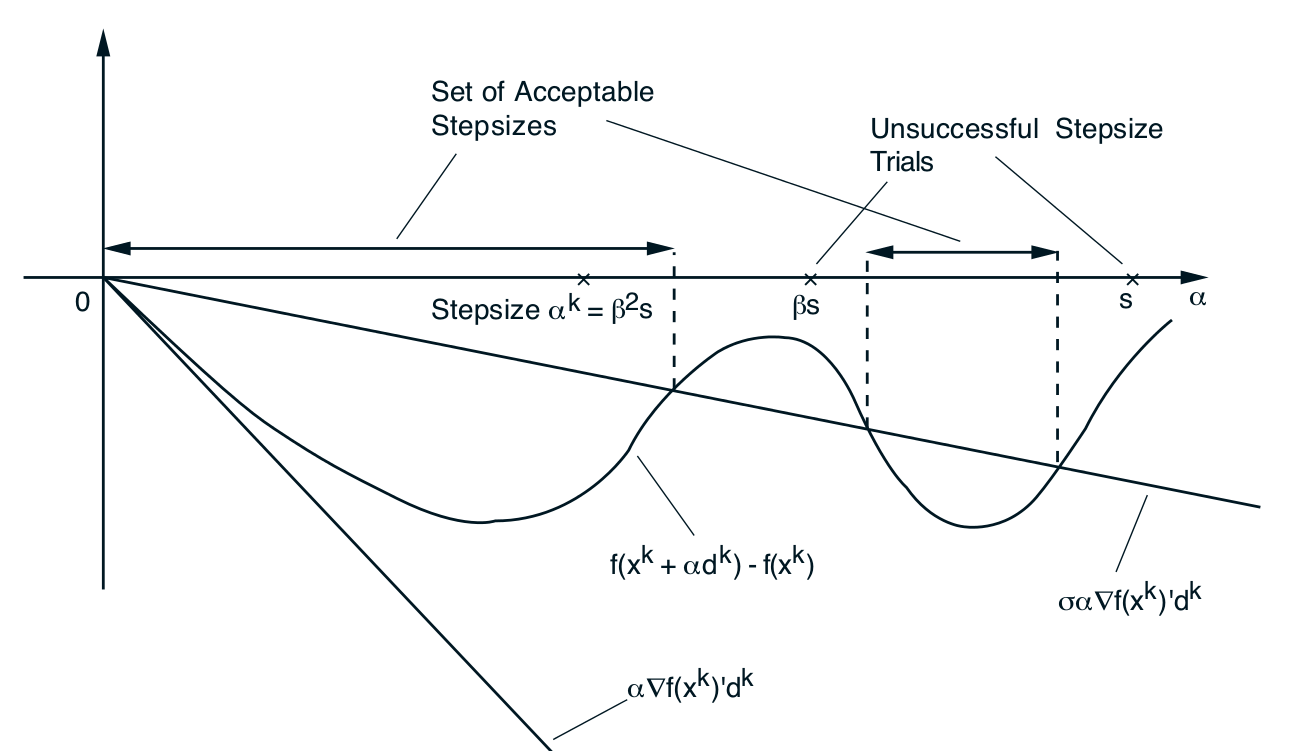
\includegraphics[width=0.8\textwidth]{armijo}
  \caption{Graphical interpretation of Armijo rule.\label{fig:armijo}}
\end{figure}


\summary{Termination of Gradient Methods}\label{s:termination}

Gradient methods are not automatically convergent, so we need some stopping criterion.  The standard
approach is to terminate iteration based on the norm of the gradient:
\begin{equation*}
  \lVert \nabla f(\kth{x}) \rVert \leq \epsilon,
\end{equation*}
for some reasonable \(\epsilon > 0\).  Since the absolute sizes of the gradients are not
neccessarily meaningful, a better criterion is
\begin{equation*}
  \frac{\lVert \nabla f(\kth{x}) \rVert}{\lVert \nabla f(\kth[0]{x}) \rVert} \leq \epsilon.
\end{equation*}
Assuming we have diagonal scaling, we can also use
\(\lVert \kth{D} \nabla f(\kth[0]{x}) \rVert \leq \epsilon\).

If \(\nabla^2 f(x)\) is positive definite, we have a strongly convex problem, and the norm of the
gradient actually bounds the distance to a local minimum \(\enVert{x - x^*}\).


%%%%%%%%%%%%%%%%%%%%%%%%%%%%%%%%%%%%%%%%%%%%%%%%%%%%%%%%%%%%%%%%%%
\section{Convergence Analysis}

\summary{Gradient Related Condition}\label{s:gradient-related-condition}

A sequence of descent directions \(\{\kth{d}\}\) is called \emph{gradient related} to a step
sequence \(\{\kth{x}\}\), if for any subsequence \(\{\kth{x}\}_{k \in \mathcal{K}}\) converging to a
nonstationary point, the corresponding subsequence \(\{\kth{d}\}_{k \in \mathcal{K}}\) is bounded
and satisfies
\begin{equation*}
  \limsup_{k \in \mathcal{K} \to \infty} \T{\nabla f(\kth{x})} \kth{d} < 0.
\end{equation*}
The interpretation of this is that in the limit, \(\kth{d}\) is still a descent direction (see
Summary~\ref{s:gradient-methods}).

This is, for example, satisfied for \(\kth{d} = -\kth{D}\nabla f(\kth{x})\), when the eigenvalues of
\(\kth{D}\) are bounded between zero and a positive constant.  It fails if the directions get more
and more orthogonal to the gradient; a counterexample would be a sequence which oscillates in the
limit, due to a badly chosen step size (there, all finite directions are descent directions, but
they get ``worse'' in the limit).


\summary{Descent Lemma}\label{s:descent-lemma}

Let \(f: \RR^n \to \RR\) have an \(L\)-Lipschitz continuous gradient.  Then for all \(x, y\), we
have the following quadratic upper bound on the objective function around \(x\):
\begin{equation*}
  f(y) \leq f(x) + \iprod{\nabla f(x)}{y - x} + \frac{L}{2}\enVert{y - x}^2,
\end{equation*}
Proof: let \(g(t) = f(x + t(y - x))\), so that \(g(0) = f(x)\) and \(g(1) = f(y)\). Then
\begin{align*}
  f(y) &= f(x) + f(y) - f(x) \\
       &= f(x) + g(1) - g(0) \\
       &= f(x) + \int_0^1 g'(t) \dif t \\
       &= f(x) + \int_0^1 \T{\nabla f(x + t(y - x))} (y - x) \dif t \\
       &= f(x) + \int_o^1 \iprod{\nabla f(x) + (f(x) + t(y - x)) - \nabla f(x)}{y - x} \dif t \\
       &= f(x) + \int_0^1 \iprod{\nabla f(x)}{y - x} \dif t
         + \int_0^1 \iprod{\nabla f(x + t(y - x)) - \nabla f(x)}{y - x} \dif t \\
       &\overset{(1)}{\leq} f(x) + \iprod{\nabla f(x)}{y - x}
         + \int_0^1 \enVert[1]{\nabla f(x + t(y - x)) - \nabla f(x)}\! \cdot \enVert[1]{y - x} \dif t \\
       &\overset{(2)}{\leq} f(x) + \iprod{\nabla f(x)}{y - x} + \enVert[1]{y - x} \int_0^1 Lt\enVert[1]{y - x} \dif t \\
       &= f(x) + \iprod{\nabla f(x)}{y - x} + \frac{L}{2}\enVert[1]{y - x}^2,
\end{align*}
where (1) is an application of the Cauchy-Schwarz theorem
(\(\langle x, y \rangle \leq \enVert{x} \cdot \enVert{y}\)), and (2) follows from Lipschitz
continuity of the gradient (Summary~\ref{s:lipschitz-continuity}):
\begin{align*}
  \enVert{\nabla f(x + t(y - x)) - \nabla f(x)} &\leq L \enVert{x + t(y - x) - x} \\
                                                &= L \enVert{t(y - x)} \\
                                                &= Lt \enVert{y - x}.
\end{align*}

\summary{Interpretation of Descent Lemma}\label{s:descent-lemma-interpretation}

We can express the lemma in terms of a step sequence \(\{\kth{x}\}\) by substituting
\(\{x \mapsto \kth{x}, y \mapsto x\}\):
\begin{equation*}
  f(x) \leq f(\kth{x}) + \T{\nabla f(\kth{x})}(x - \kth{x}) + \frac{L}{2}\enVert[1]{x - \kth{x}}^2.
\end{equation*}
This is actually a local upper bound of \(f\) at \(x\) by a quadratic function, which we can
optimize analytically:
\begin{gather*}
  \nabla f(\kth{x}) + L (x - \kth{x}) \overset{!}{=} 0 \\
  \quad \Rightarrow x = \kth{x} - \frac{1}{L} \nabla f(\kth{x})
\end{gather*}
Convergent step size methods relate to this fact.

The upper bound of provided by the descent lemma is a global upper bound on the second-order error
of the Taylor expansion.  In this way, it is exactly dual to \(\mu\)-strong convexity
(Summary~\ref{s:strong-convexity}) in the differential formulation, which provides the analog
lower bound.


\summary{Convergence with Constant Step Size}\label{s:convergence-constant}

Assume \(f\) is Lipschitz continuous, and \(\{\kth{x}\}\) is a sequence generated by a gradient
method with gradient related \(\kth{d} \neq 0\).  By that we have
\begin{align*}
  f(\kth{x} + \kth{\alpha}\kth{d}) - f(\kth{x})
  &\leq \overbrace{\T{\nabla f(\kth{x})} \kth{d}}^{< 0} \kth{\alpha} +
    \frac{1}{2} (\kth{\alpha})^2 L \enVert[1]{\kth{d}}^2 \\
  &= \underbrace{\kth{\alpha} \left( \frac{1}{2} \kth{\alpha} L \enVert[1]{\kth{d}}^2
    - \envert[1]{\nabla f(\kth{x}) \kth{d}} \right)}_{A}.
\end{align*}
We first calculate the optimal step size \(\kth{\bar{\alpha}} = \min_{\kth{\alpha}} A\):
\begin{gather*}
  \dpd{A}{{\kth{\alpha}}} = (\kth{\alpha})^2 L \enVert[1]{\kth{d}}^2 - \envert[1]{\T{\nabla
                            f(\kth{x})} \kth{d}} \overset{!}{=} 0 \\
  \Rightarrow \kth{\bar{\alpha}} = \enVert[1]{\kth{d}} - \frac{\envert[1]{\T{\nabla
                       f(\kth{x})} \kth{d}}}{(\kth{\alpha})^2 L \enVert[1]{\kth{d}}^2}
\end{gather*}
Then, for general \(\kth{\alpha}\) with
\(\epsilon \leq \kth{\alpha} \leq (2 - \epsilon)\kth{\bar{\alpha}}\), we have
\begin{align*}
  &f(\kth{x} + \kth{\alpha}\kth{d}) - f(\kth{x}) \\
  &\qquad \leq \kth{\alpha} \left( \frac{1}{2} L \enVert[1]{\kth{d}}^2
    - \envert[1]{\T{\nabla f(\kth{x})} \kth{d}} \right) \\
  &\qquad \leq \kth{\alpha} \left( \frac{1}{2} (2 - \epsilon)\; \frac{\envert[1]{\T{\nabla
    f(\kth{x})} \kth{d}}}{(\kth{\alpha})^2 L \enVert[1]{\kth{d}}^2} L \enVert[1]{\kth{d}}^2
    - \envert[1]{\T{\nabla f(\kth{x})} \kth{d}} \right) \\
  &\qquad = \kth{\alpha} \left( \envert[1]{\T{\nabla f(\kth{x})} \kth{d}}
    - \frac{\epsilon}{2} \envert[1]{\T{\nabla f(\kth{x})} \kth{d}}
    - \envert[1]{\T{\nabla f(\kth{x})} \kth{d}} \right) \\
  &\qquad = \kth{\alpha} \underbrace{\left( -\frac{\epsilon}{2}\envert[1]{\T{\nabla f(\kth{x})} \kth{d}}
    \right)}_{\leq 0};
\end{align*}
and by the reverse,
\begin{align*}
  f(\kth{x}) - f(\kth{x} - \kth{\alpha}\kth{d})
  &\geq \kth{\alpha} \left(\frac{\epsilon}{2}\envert[1]{\T{\nabla f(\kth{x})} \kth{d}} \right) \\
  &\geq \frac{\epsilon^2}{2}\envert[1]{\T{\nabla f(\kth{x})} \kth{d}},
\end{align*}
where the last step results from the assumption about \(\kth{\alpha}\).  Thus,
\(f(\kth{x}) \geq f(\kth[k+1]{x}) \geq \cdots \); in each step, the function is decreased by an
amount of at least \(\frac{\epsilon^2}{2}\envert[1]{\T{\nabla f(\kth{x})} \kth{d}}\).

Convergence to a stationary point follows by contradiction: assume a subsequence
\(\{\kth{x}\}_{k \in \mathcal{K}}\) converged to a point \(\bar{x}\) which is non-stationary (ie.,
for which \(\nabla f(\bar{x}) \neq 0\)).  From above, we know that
\begin{equation*}
  f(\kth{x} + \kth{\alpha}\kth{d}) - f(\kth{x}) \to 0
\end{equation*}
(assuming \(f\) is bounded below), and by that
\begin{equation*}
\envert[1]{\T{\nabla f(\kth{x})} \kth{d}} \to 0  
\end{equation*}
This would however contradict to \(\kth{d}\) being gradient related, since it implies
\begin{equation*}
  \limsup_{k \in \mathcal{K} \to \infty} \T{\nabla f(\kth{x})} \kth{d} = 0
\end{equation*}
Therefore, every accumulation point \(\bar{x}\) of \(\{\kth{x}\}\) must be stationary
(\(\nabla f(\bar{x}) = 0\)).


\summary{Convergence with Armijo Rule}\label{s:convergence:armijo}
\todo{TODO}


\summary{Convergence Rates}\label{s:convergence-rates}

Important for practical problems, to compare different algorithms.  Is usually measured in terms of
a step-dependent error function \(e: \RR^n \to \RR\) with \(e(x^*) = 0\).  Common choices are
\begin{gather*}
  e(x) = \enVert[1]{x - x^*}, \text{ or } \\
  e(x) = f(x) - f(x^*)
\end{gather*}
We are interested in the asymptotic behaviour of \(e\), in terms of how much better the method
improves for every step.  We have:
\begin{enumerate}
\item Sublinear convergence, if
  \begin{equation*}
    \limsup_{k \to \infty} \frac{e(\kth[k+1]{x})}{e(\kth{x})} = 1.
  \end{equation*}
\item Linear convergence, if
  \begin{equation*}
    \limsup_{k \to \infty}
    \frac{e(\kth[k+1]{x})}{e(\kth{x})} \leq \beta \in (0, 1).
  \end{equation*}
\item Superlinear convergence, if
  \begin{equation*}
    \limsup_{k \to \infty} \frac{e(\kth[k+1]{x})}{e(\kth{x})} = 0.
  \end{equation*}
  (which does not imply that the method does not converge!)
\end{enumerate}
Alternatively, we can compare \(e\) to a standard sequence of powers: if there exist \(q > 0\),
\(\beta \in (0, 1)\), and \(p \geq 1\) such that for all \(k\)
\begin{equation*}
  e(\kth{x}) \leq q \beta^{p^k},
\end{equation*}
we have linear convergence if \(p = 1\), and superlinear convergence of order \(p\) if \(p > 1\).
The latter is equivalent to
\begin{equation*}
  \limsup_{k \to \infty} \frac{e(\kth[k+1]{x})}{e(\kth{x})^p} < \infty.
\end{equation*}
\todo{derivations for some rates? analysis of quadratic model?}


%%%%%%%%%%%%%%%%%%%%%%%%%%%%%%%%%%%%%%%%%%%%%%%%%%%%%%%%%%%%%%%%%%
\section{Newton's Method and Variants}

\summary{Basic Idea}\label{s:newtons-basics}

A second order method, which is one of the fastest gradient methods.  We generate the sequence
\(\{\kth{x}\}\) based on
\begin{equation*}
  \kth[k+1]{x} = \kth{x} - \kth{\alpha}\left( \nabla^2 f(\kth{x}) \right)^{-1} \nabla f(\kth{x}),
\end{equation*}
where we assume that the direction \((\nabla^2 f(\kth{x}))^{-1} \nabla f(\kth{x}\) is
defined and a descent direction.

Close to a local minimum, \(\kth{\alpha} = 1\) will work well. However, when we are far from a local
minimum, we run into problems:
\begin{enumerate}
\item The Hessian can be singular~-- we what are reasonable approximations in this case?
\item The Hessian is convex~-- it attracts local maxima as well as minima.  Thus, we must choose the
  step size carfully.
\item The direction might not be a descent direction.
\end{enumerate}
Variants of the method deal with this, to ensure convergence globally while maintaining the fast
convergence rate.


\summary{Derivation of Newton's Method from Taylor Expansion}\label{s:newton-method-derivation}

By Taylor approximation: Given a point \(\kth{x}\), we can approximate a function
\(f \in \mathcal{C}^2\) locally as
\begin{equation*}
  \kth{T}(x) = f(\kth{x}) + \T{\nabla f(\kth{x})}(x - \kth{x})
  + \frac{1}{2} \T{(x - \kth{x})} \nabla^2 f(\kth{x})(x - \kth{x}).
\end{equation*}
Compare this to the descent lemma (Summary~\ref{s:descent-lemma-interpretation})~-- there,
\(\nabla^2 f\) is approximated by \(L\), with some transformation of the metric.

We can analytically minimize this approximation, which gives the stated update rule:
\begin{align*}
  0 \overset{!}{=} \nabla \kth{T}(\kth[k+1]{x})
      &= \nabla f(\kth{x}) + \nabla^2 f(\kth{x})(\kth[k+1]{x} - \kth{x}) \\
  \nabla^2 f(\kth{x})(\kth[k+1]{x} - \kth{x}) &= -\nabla f(\kth{x}) \\
  (\kth[k+1]{x} - \kth{x}) &= -(\nabla^2 f(\kth{x}))^{-1} \nabla f(\kth{x}) \\
  \kth[k+1]{x} &= \kth{x} - (\nabla^2 f(\kth{x}))^{-1} \nabla f(\kth{x}).
\end{align*}


\summary{Relation of Newton's Method to Equation Solving}\label{s:newton-equations}

The general for of Newton's method is not used for optimization, but for solving equations of the
form \(g(x) = 0\), where \(g: \RR^n \to \RR^n \in \mathcal{C}^1\).  For this problem, the method has
the form
\begin{equation*}
  \kth[k+1]{x} = \kth{x} - (\T{\nabla g(\kth{x})})^{-1} g(\kth{x}).
\end{equation*}
A method converging to a stationary point results from setting \(g(x) = \nabla f(x)\), implying a
symmetric matrix \(\T{\nabla g(x)} = \nabla^2 f(x)\).


\summary{Scale Invariance}\label{s:newton-scale}

Newton's method has the property that it is invariant under affine coordinate changes; i.e. if we
used a transformation of variables \(Sy = x\), such that \((f \circ S)(y) = f(x)\), where \(S\) is a
nonsingular affine transformation, the generated steps will remain the same.  Proof: First, observe
that by chain rule,
\begin{align*}
  \nabla (f \circ S)(y) &= \T{S}(\nabla f \circ S)(y), \\
  \nabla^2 (f \circ S)(y) &= \T{S}(\nabla^2 f \circ S))(y)S.
\end{align*}
Now, the second-order approximation of \(f \circ S\) around \(\kth{y}\) becomes
\begin{align*}
  \kth{T}(y) &= (f \circ S)(\kth{y}) + \T{\nabla (f \circ S)(\kth{y})}(y - \kth{y}) \\
             &\quad + \frac{1}{2} \T{(y - \kth{y})} \nabla^2 (f \circ S)(\kth{y}) (y - \kth{y}) \\
             &= (f \circ S)(\kth{y}) + \T{(\T{S}(\nabla f \circ S)(\kth{y}))}(y - \kth{y}) \\
             &\quad + \frac{1}{2} \T{(y - \kth{y})}
               \T{S}(\nabla^2 f \circ S)(\kth{y})S (y - \kth{y}).
\end{align*}
We can then set \(\kth[k+1]{y}\) as the minimizer of \(\kth{T}\) to get the update rule, like above:
\begin{align*}
  & & 0 \overset{!}{=} \nabla \kth{T}(\kth[k+1]{y}) &= \T{S}(\nabla f \circ S)(\kth{y})
                                                      + \T{S}(\nabla^2 f \circ S)(\kth{y})S
                                                      (\kth[k+1]{y} - \kth{y}) \\
  & & 0 &= S(\kth[k+1]{y} - \kth{y}) + \left( \T{S}(\nabla^2 f \circ S)(\kth{y}) \right)^{-1}
          \T{S}(\nabla f \circ S)(\kth{y}) \\
  & & &= S(\kth[k+1]{y} - \kth{y}) + \left( (\nabla^2 f \circ S)(\kth{y}) \right)^{-1} (\T{S})^{-1}
          \T{S}(\nabla f \circ S)(\kth{y}) \\
  & & S\kth[k+1]{y} &= S\kth{y} - \left( (\nabla^2 f \circ S)(\kth{y}) \right)^{-1}
                      (\nabla f \circ S)(\kth{y}) \\
  & & &= S\kth{y} - \left( \nabla^2 f(S\kth{y}) \right)^{-1}
                      \nabla f(S\kth{y}).
\end{align*}
Here we can substitute back to get
\begin{equation*}
  \kth[k+1]{x} = \kth{x} - \nabla^2 f(\kth{x})^{-1} \nabla f(\kth{x}),
\end{equation*}
which is equivalent to the above result.

\summary{Local convergence}\label{s:newton-local-convergence}

For a local optimum \(x^*\) of \(f\), we must have \(\nabla f(x^*) = 0\), or, by the above relation
to equation solving, \(g(x^*) = 0\).  Now, suppose \(\kth{x} \to x\) and \(\nabla f(x^*)\) is
nonsingular.  Expanding \(g\) around \(x^*\), we get
\begin{equation*}
  0 = g(x^*) = g(\kth{x}) + \T{\nabla g(\kth{x})} (x^* - \kth{x}) + o\!\del[1]{\,\enVert[1]{x^* - \kth{x}}};
\end{equation*}
multiplying from the left with \((\T{\nabla g(\kth{x})})^{-1}\), this is
\begin{gather*}
  \kth{x} - x^* - (\T{\nabla g(\kth{x})})^{-1} g(\kth{x}) = \kth[k+1]{x} - x^* = o\!\del[1]{\,\enVert[1]{x^* - \kth{x}}} \\
  \Rightarrow \quad \lim_{k \to \infty} \frac{\enVert[1]{\kth[k+1]{x} - x^*}}{\enVert[1]{\kth{x} - x^*}} = 0,
\end{gather*}
therefore we have superlinear convergence.


\summary{Global Convergence by Diagonal Modifications}\label{s:newton-global-convergence}

To solve the problems mentioned above, when we are far away from an optimum, we can add a diagonal
matrix \(\kth{\Delta}\) to the Hessian, such that \(\nabla^2 f(\kth{x}) + \kth{\Delta} \succ 0\).
In that way, the Newton equation
\begin{equation*}
  \left( \nabla^2 f(\kth{x}) + \kth{\Delta} \right) \kth{d} = -\nabla f(\kth{x})
\end{equation*}
can be solved, and \(\kth{d}\) is a descent direction.  Some possibilities for \(\kth{\Delta}\) are
simply a large enough multiple of \(I\), or more advanced methods like modified Cholesky
factorization\footnote{\url{https://www.gnu.org/software/gsl/manual/html_node/Modified-Cholesky-Decomposition.html}}
or a combination of a dampening factor with a trust
region\footnote{\url{https://en.wikipedia.org/wiki/Trust_region}}.


%%%%%%%%%%%%%%%%%%%%%%%%%%%%%%%%%%%%%%%%%%%%%%%%%%%%%%%%%%%%%%%%%%
\section{Least Squares Optimization \& Model Fitting}

\summary{General Form}\label{s:least-squares}

We want to minimize
\begin{equation*}
  f(x) = \frac{1}{2} \enVert[1]{g(x)}^2 = \frac{1}{2} \sum_i g_i(x)^2,
\end{equation*}
for a continuously differentiable function \(g\) with components \(g_i\), which can be linear or
nonlinear.  This is equivalent to solving the problem \(g(x) = 0\), a possibly overdetermined
system.

Often, a least squares problem is a model fitting problem, where
\begin{equation*}
  g_i(\theta) = h(x_i, \theta) - \hat{y}_i
\end{equation*}
is the loss for a single sample for a model function \(h\) with parameters \(\theta\), samples
\(x_i\), and targets~\(\hat{y}_i\).


\summary{Gauss-Newton Method}\label{s:gauss-newton-method}

To get a step method, we replace \(g(x)\) by a local approximation around \(\kth{x}\):
\begin{equation*}
  \tilde{g}(x, \kth{x}) = g(\kth{x}) + \T{\nabla g(\kth{x})}(x - \kth{x}),
\end{equation*}
which yields
\begin{align*}
  \tilde{f}(x, \kth{x})
    &= \frac{1}{2} \enVert{\tilde{g}(x, \kth{x})}^2 \\
    &= \frac{1}{2} \T{\tilde{g}(x, \kth{x})}\tilde{g}(x, \kth{x}) \\
    &= \frac{1}{2} \left( \T{g(\kth{x})} + \T{(x - \kth{x})}\nabla g(\kth{x}) \right)
      \left( g(\kth{x}) + \T{\nabla g(\kth{x})}(x - \kth{x}) \right) \\
    &= \frac{1}{2} \Big( \T{g(\kth{x})}g(\kth{x}) \\
    &\qquad + \T{g(\kth{x})}\T{\nabla g(\kth{x})}(x - \kth{x}) + \T{(x - \kth{x})}\nabla
      g(\kth{x})g(\kth{x}) \\
    &\qquad + \T{(x - \kth{x})}\nabla g(\kth{x})\T{\nabla g(\kth{x})}(x - \kth{x}) \Big) \\
    &= \frac{1}{2} \enVert[1]{g(\kth{x})}^2 + 2\T{(x - \kth{x})} \nabla g(\kth{x})g(\kth{x}) \\
    &\qquad + \T{(x - \kth{x})} \nabla g(\kth{x})\T{\nabla g(\kth{x})}(x - \kth{x}).
\end{align*}
(Note that \(\nabla g\), as the Jacobian, is a matrix!)  Then we can turn this into a quadratic
problem, yielding the next step as the minimum of the approximation
\begin{equation*}
  \kth[k+1]{x} \in \argmin_{x \in \RR^n} \tilde{f}(x, \kth{x}),
\end{equation*}
which we can solve as
\begin{align*}
  & & 0 &\overset{!}{=} \nabla_{\kth[k+1]{x}} f(\kth[k+1]{x}, \kth{x}) \\
  & & &= \T{\nabla g(\kth{x})} g(\kth{x})
        + \nabla g(\kth{x})\T{\nabla g(\kth{x})} (\kth[k+1]{x} - \kth{x}) \\
  % && &\qquad+ \T{(\kth[k+1]{x} - \kth{x})} \nabla g(\kth{x}) \T{\nabla g(\kth{x})} g(\kth{x}) \Big) \\
  &\Rightarrow  & \kth[k+1]{x} &= \kth{x} - \left(\nabla g(\kth{x}) \T{\nabla
                 g(\kth{x})}\right)^{-1}
                 \T{\nabla g(\kth{x})} g(\kth{x}),
\end{align*}
assuming that \(\nabla g(\kth{x}) \T{\nabla g(\kth{x})}\) is invertible.  If \(g\) is linear, this
method reduces to the Moore-Penrose pseudoinverse and solves the problem in one step.


\summary{Levenberg-Marquardt Method}\label{s:levenberg-method}

To ensure that \(\nabla g(\kth{x}) \T{\nabla g(\kth{x})}\) is invertible, and the descent direction
is actually gradient related, one can use a modified iteration scheme
\begin{equation*}
  \kth[k+1]{x} = \kth{x} - \kth{\alpha}\left(\nabla g(\kth{x}) \T{\nabla g(\kth{x})} + \kth{\delta} I\right)^{-1}
  \nabla g(\kth{x}) g(\kth{x}),
\end{equation*}
where \(\kth{\alpha}\) can be chosen by the Armijo rule, and \(\kth{\delta} > 0\) large enough.


\summary{Connection of Gauss-Newton to Newton}\label{s:newton-gauss-newton}
% bertsekas 107

The target function of a least squares problem, \(f(x) = \frac{1}{2}\enVert[0]{g(x)}^2\), with
components \(g_i\), has derivatives
\begin{align*}
  \nabla f(x) &= \T{\nabla g(x)} g(x), \\
  \nabla^2 f(x) &= \nabla g(x) \T{\nabla g(x)} + \sum_i \nabla^2 g_i(x) g_i(x).
\end{align*}
Neglecting the second-order part in the Hessian, this reduces to a form equivalent to Newton's
method, but saving the computation of the Hessian (intuitively, \(\nabla^2 g \approx (\nabla g)^2\)).


\summary{Incremental Gradient Methods}\label{s:incremental-gradient-methods}

If a least squares problem is a model fitting problem, where \(g_i(x) = z_i - h(y_i, x)\), for
samples \(y_i\), and targets and \(z_i\), we can see each \(g_i\) as a data block, and
\(g = (g_1, \ldots, g_m)\) as the data set.  (In machine learning terminology, this corresponds to
stochastic gradient descent with minibatches for ``data blocks''.)

When this data set is large, the Gauss-Newton iterations are costly (because the matrix to be
inverted becomes large).  Sometimes, for example in real-time applications, the data samples also
are not provided in advance, but only incrementally.  Therefore, we can use the following scheme to
calculate updates based on single samples:
\begin{align*}
  \kth{\xi}_0 &= \kth{x} \\
  \kth{\xi}_i &= \kth{\xi}_{i-1} - \kth{\alpha} \nabla g_i(\kth{\xi}_{i-1}) g_i(\kth{\xi}_{i-1}) \\
  \kth[k+1]{x} &= \kth{\xi}_m.
\end{align*}
This amounts to
\begin{equation*}
  \kth[k+1]{x} = \kth{x} - \kth{\alpha} \sum_i \nabla g_i(\kth{\xi}_{i-1}) g_i(\kth{\xi}_{i-1}),
\end{equation*}
where we base the update on the intermediate \(\kth{\xi}_i\) instead of using the full gradient
\begin{equation*}
  \nabla f(\kth{x}) = \sum_i \nabla g_i(\kth{x}) g_i(\kth{x}).
\end{equation*}
This converges very fast in the first iterations, but needs further restictions on the step size to
ensure global convergence.


\summary{Kalman Filter}\label{s:kalman-filter}

If the model (ie. the functions \(g_i\)) is linear, one Gauss-Newton iteration is enough to find the
least squares estimate (this amounts to the analytical solution using the Moore-Penrose
pseudoinverse).  However, we can develop an incremental method for this, avoiding the matrix
inversion.  This method is called \emph{Kalman filter}.

Suppose \(g_i(x) = z_i - C_i x_i\), with \(z_i \in \RR^r\) and \(C_i \in \RR^{r \times n}\) (the
model parameters).  We are interested in a method for finding
\begin{equation*}
  \xi_i \in \argmin_x \sum_{j=1}^{i} \lambda^{i-j} \enVert[1]{z_j - C_j x}^2.
\end{equation*}
The optimal solution is then \(x^* = \xi_m\).  For \(\lambda = 1\), this is the least squares fit;
for \(\lambda < 1\), we ``decay'' the importance of ``older'' samples.  The sequence of \(\xi_i\)
can be generated iteratively by
\begin{align*}
  \xi_i &= \xi_{i-1} + H_i^{-1}\T{C_i}(z_i - C_i \xi_{i-1}), \quad\text{with} \\
  H_i &= \lambda H_{i-1} + \T{C_i}C_i, \\
  H_0 &= 0,\quad \xi_0 \text{ arbitrary}.
\end{align*}
(here \(H_i\) and \(C_i\) are relatively small, compared to \(\nabla g(\kth{x})\).)

Example: for a linear model \(x(t) = l + ft\), with parameters \(f, l\), we use \(C = [1, t]\).


\summary{Extended Kalman Filter}\label{s:extended-kalman-filter}

If the \(g_i\) are nonlinear, we can use a linearization at the last available iteration
\(\xi_{i-1}\) to get the \emph{extended Kalman filter}:
\begin{gather*}
  \tilde{g}_i(x, \xi_{i-1}) = g_i(\xi_{i-1}) + \T{\nabla g_i(\xi_{i-1})}(x - \xi_{i-1}), \\
  \xi_i \in \argmin_x \sum_{j=1}^{i} \lambda^{i-j} \enVert[1]{\tilde{g}_j(x, \xi_{i_1})}.
\end{gather*}
The iteration scheme stays the same, but the model parts must be adapted to
\begin{align*}
  \tilde{z}_i &= \tilde{g}_i(z_i, \xi_{i-1}), \\
  C_i &= - \T{\nabla g_i(\xi_{i-1})}.
\end{align*}


%%%%%%%%%%%%%%%%%%%%%%%%%%%%%%%%%%%%%%%%%%%%%%%%%%%%%%%%%%%%%%%%%%
\section{Accelerated Gradient Methods}

\optionalsummary{General Lower Bounds for Convex Functions}\label{s:convex-lower-bound}

A general first-order gradient method generates steps of the form
\begin{equation*}
  \kth[k+1]{x} \in \kth[0]{x} + \Span \{\nabla f(\kth[0]{x}), \ldots, \nabla f(\kth{x})\}.
\end{equation*}
We can give the following general lower bounds for convex functions:
\begin{itemize}
\item Smooth convex functions: for any \(k\) with \(1 \leq k \leq \frac{1}{2}(n - 1)\), \(L > 0\),
  and \(\kth[0]{x} \in \RR^n\), there is a function \(f \in \Lip{L}{\infty}{1}\) such that for any
  first order method we have
  \begin{enumerate}
  \item \(\displaystyle \enVert[1]{\kth{x} - x^*} \geq \frac{1}{8} \enVert[1]{\kth[0]{x} - x^*}\)
  \item \(\displaystyle f(\kth{x}) - f(x^*) \geq \frac{3L \enVert[1]{\kth[0]{x} - x^*}}{32 (k+1)^2}\),
  \end{enumerate}
\item Strongly convex functions: for any \(\kth[0]{x} \in \RR^n\), \(\mu > 0\), and \(L > \mu\),
  there is a function \(f \in \Strong{\mu}{L}{\infty}{1}\) such that for any first order method we
  have
  \begin{enumerate}
  \item \(\displaystyle \enVert[1]{\kth{x} - x^*}^2 \geq
    \left( \frac{\sqrt{L/\mu} - 1}{\sqrt{L/\mu} + 1} \right)^k \enVert[1]{\kth[0]{x} - x^*}^2\)
  \item \(\displaystyle \displaystyle f(\kth{x}) - f(x^*) \geq \frac{\mu}{2}
    \left( \frac{\sqrt{L/\mu} - 1}{\sqrt{L/\mu} + 1} \right)^{2k} \enVert[1]{\kth[0]{x} - x^*}^2\)
  \end{enumerate}
  Here, the value \(L / \mu \geq 1\) is called the \emph{condition number} of the function and often
  abbreviated as \(Q_f\).
\end{itemize}


\summary{\texorpdfstring{\(Q\)}{Q}-Conjugacy}\label{s:q-conjugacy}

Given a positive definite matrix \(Q\), a set of nonzero vectors
\(\kth[0]{d}, \ldots, \kth[k-1]{d}\) are called \emph{\(Q\)-conjugate} if for all \(i \neq j\)
\begin{equation*}
  \T{(\kth[i]{d})} Q \kth[j]{d} = 0.
\end{equation*}
We can interpret this as orthogonality in the metric given by \(Q\), which induces an inner product
\(\langle \cdot \rangle_Q\).  Since the \(\kth[i]{d}\) are linearly independent in the \(Q\)-metric,
they are also linearly independent in the normal metric.

Given a set of linearly independent vectors \(\kth[0]{\xi}, \ldots, \kth{\xi}\), we can construct a
set of mutually \(Q\)-conjugate vectors \(\kth[0]{d}, \ldots, \kth{d}\) spanning the same space by
the \emph{Gram-Schmidt procedure}.  Therefore, we first define the projection operator onto a vector
\(d\) (in the \(Q\)-metric):
\begin{equation*}
  \proj_d(\xi) = \frac{\langle d, \xi \rangle_Q}{\langle d, d \rangle_Q} d
  = \frac{\T{d} Q \xi}{\T{d} Q d} d.
\end{equation*}
Then we can iteratively orthogonalize the \(\kth[i]{\xi}\) by removing all projections on the already
orthogonalized ones:
\begin{align*}
  \kth[0]{d} &= \kth[0]{\xi} \\
  \kth[k]{d} &= \kth[k]{\xi} - \sum_{j=0}^{k-1} \proj_{\kth[j]{d}}(\kth[k]{\xi}) \\
             &= \kth[k]{\xi} - \sum_{j=0}^{k-1}
               \frac{\T{(\kth[j]{d})} Q \kth[k]{\xi}}{\T{(\kth[j]{d})} Q \kth[j]{d}} \kth[j]{d}.
\end{align*}


\summary{Conjugate Direction Methods}\label{s:conjugate-direction-methods}

For \emph{quadratic problems} of the form
\begin{equation*}
  \min_{x \in \RR^n} f(x) = \frac{1}{2} \T{x}Qx - \T{b}x,
\end{equation*}
these methods accelerate the slow convergence of gradient methods, while still avoiding the overhead
of second-order methods, like Newton's.  Originally, they were developed for symmetric and positive
definite \(Q\), but they also work for solving linear systems of the form \(Qx = b\), where \(Q\) is
not neccessarily symmetric, but just invertible.

For a given set of \(Q\)-conjugate descent directions \(\kth[0]{d}, \ldots, \kth{d}\), the conjugate
direction method minimizing a quadratic function \(f: \RR^n \to \RR\) is given by the gradient
method
\begin{equation*}
  \kth[k+1]{x} = \kth{x} - \kth{\alpha}\kth{d},
\end{equation*}
where \(\kth{\alpha}\) is obtained by line minimization and \(\kth[0]{x}\) is arbitrary.

This method generates steps which minimize the function over a sequence of expanding linear
submanifolds \(\kth{M}\) of the domain of \(f\):
\begin{equation*}
  \kth[k+1]{x} = \argmin_{x \in \kth{M}} f(x),
\end{equation*}
where
\begin{equation*}
  \kth{M} = \kth[0]{x} + \Span (\kth[0]{d}, \ldots, \kth{d}).
\end{equation*}
Since by construction, the \(\kth[i]{d}\) span the same space as the \(\kth[i]{x}\), \(\kth[n]{x}\)
minimizes the function over its whole domain; hence, the method terminates after at most \(n\)
steps (in theory, assuming exact arithmetic).


\summary{Conjugate Gradient Method}\label{s:conjugate-gradient-method}

The conjugate gradient method (CG) is the most important conjugate direction method for quadratic
problems.  The step scheme is
\begin{equation*}
  \kth[k+1]{x} = \kth{x} + \kth{\alpha}\kth{d},
\end{equation*}
where \(\kth{\alpha}\) is chosen by line minimization, and the descent directions are obtained by
simply applying the Gram-Schmidt procedure on the gradient vectors at the successive steps: we set
\(\kth[i]{\xi} = -\kth[i]{g}\) for
\begin{equation*}
  \kth{g} = \nabla f(\kth{x}) = Q \kth{x} - b,
\end{equation*}
and calculate the descent directions \(\kth[i]{d}\) as stated above:
\begin{align*}
  \kth[0]{d} &= -\kth[0]{g}, \\
  \kth[k]{d} &= -\kth[k]{g} + \sum_{j=0}^{k-1}
               \frac{\T{(\kth[k]{g})} Q \kth[j]{d}}{\T{(\kth[j]{d})} Q \kth[j]{d}} \kth[j]{d}.
\end{align*}
Since all but one of the coefficients are zero, the sum can be simplified to
\begin{equation*}
  \kth{d} = -\kth{g} + \kth{\beta}\kth[k-1]{d},
\end{equation*}
where \(\kth{\beta}\) is given by
\begin{equation*}
  \kth{\beta} = \frac{\T{(\kth{g})}\kth{g}}{\T{(\kth[k-1]{g})}\kth[k-1]{g}}.
\end{equation*}

This method terminates with an optimal solution after at most \(n\) steps (as argued above), and is
an optimal first order method for quadratic problems, for which we have the easy characterization
\(L = \lambda_{\text{max}}(Q)\) and \(\mu = \lambda_{\text{min}}(Q)\): if \(Q\) is positive
definite, and \(0 \preceq \mu \preceq Q \preceq L\), then we have a strongly convex problem with
\begin{equation*}
  \enVert[1]{\kth{x} - x^*}^2 \leq 2\sqrt{L/\mu} \left( \frac{\sqrt{L/\mu}-1}{\sqrt{L/\mu}+1} \right)^{2k}
  \enVert[1]{\kth[0]{x} - x^*}^2.
\end{equation*}
If \(Q\) is just positive semidefinite with \(0 \preceq Q \preceq L\), we have a smooth problem with
\begin{equation*}
  f(\kth{x}) - f(x^*) \leq \frac{L \enVert[1]{\kth[0]{x} - x^*}^2}{2 (2k + 1)^2}.
\end{equation*}


\summary{Application of CG to Nonlinear Problems}\label{s:conjugate-gradient-nonlinear}

For general minimization problems, we can adapt the idea of the above method as follows:
\(\kth{\alpha}\) is still chosen by line minimization, but we generate the descent directions via
\begin{equation*}
  \kth{d} = -\nabla f(\kth{x}) + \kth{\beta}\kth[k-1]{d},
\end{equation*}
where \(\kth{\beta}\) is computed as
\begin{equation*}
  \kth{\beta} = \frac{\T{\nabla f(\kth{x})}(\nabla f(\kth{x}) - \nabla f(\kth[k-1]{x}))}{
    \T{\nabla f(\kth[k-1]{x})} \nabla f(\kth[k-1]{x})}.
\end{equation*}
Here, we can't anymore say anything about convergence.  It might be neccessary to sometimes restart
the procedure with \(\kth{\beta} = 0\).


\summary{Heavy Ball Method}\label{s:heavy-ball-method}

In machine learning terminology, this is the same as using a \emph{momentum term}.  We use a
multi-step iteration scheme
\begin{equation*}
  \kth[k+1]{x} = \kth{x} - \kth{\alpha} \nabla f(\kth{x}) + \kth{\beta}(\kth{x} - \kth[k-1]{x}).
\end{equation*}

The idea behind this comes from the physical system of a ``heavy ball'' with friction: we descretize
the differential equation (for a given \(f\)):
\begin{equation*}
  \ddot{x}(t) + \gamma\dot{x}(t) + \nabla f(x(t)) = 0
\end{equation*}
using finite differences:
\begin{align*}
  \ddot{x}(t) &\approx \frac{\kth[k+1]{x} - 2\kth{x} + \kth[k-1]{x}}{h^2}, \\
  \dot{x}(t) &\approx \frac{\kth[k+1]{x} - \kth{x}}{h}, \\
  \nabla f(x(t)) &\approx \nabla f(\kth{x}).
\end{align*}
We can arrange these terms to get the above form, where \(\alpha\) and \(\beta\) are to be chosen.
If \(f\) is a quadratic problem, we can solve for them analytically: let
\begin{equation*}
  \kth[k+1]{x} = \kth{x} - \kth{\alpha} (\underbrace{Q\kth{x} - b}_{\kth{r}})
  + \kth{\beta}(\underbrace{\kth{x} - \kth[k-1]{x}}_{\kth{p}}).
\end{equation*}
Now, we insert this back into the function:
\begin{align*}
  (\kth{\alpha}, \kth{\beta}) &= \argmin_{\alpha, \beta}
  \frac{1}{2} \T{(\kth{x} - \alpha\kth{r} + \beta\kth{p})}Q(\kth{x} - \alpha\kth{r} + \beta\kth{p}) \\
  &\phantom{\argmin_{\alpha, \beta}}\qquad - \T{b}(\kth{x} - \alpha\kth{r} + \beta\kth{p}).
\end{align*}
The right hand side has a gradient of
\begin{equation*}
  \begin{pmatrix}
    -\T{(\kth{r})}Q(\kth{x} - \alpha\kth{r} + \beta\kth{p}) + \T{b}\kth{r} \\
    \phantom{-}\T{(\kth{p})}Q(\kth{x} - \alpha\kth{r} + \beta\kth{p}) + \T{b}\kth{p}
  \end{pmatrix},
\end{equation*}
which when set to zero leads to a linear system in \(\alpha\), \(\beta\) with solutions
\begin{align*}
  \kth{\alpha} &= \frac{\enVert[1]{\kth{r}}^2 \langle Q\kth{p}, \kth{p} \rangle -
                 \langle \kth{r}, \kth{p} \rangle \langle Q\kth{r}, \kth{p} \rangle}{
                 \langle Q\kth{r}, \kth{r} \rangle \langle Q\kth{p}, \kth{p} \rangle
                 - \langle Q\kth{r}, \kth{p} \rangle^2},\\
  \kth{\beta} &= \frac{\enVert[1]{\kth{r}}^2 \langle Q\kth{r}, \kth{p} \rangle -
                 \langle \kth{r}, \kth{p} \rangle \langle Q\kth{r}, \kth{r} \rangle}{
                 \langle Q\kth{r}, \kth{r} \rangle \langle Q\kth{p}, \kth{p} \rangle
                 - \langle Q\kth{r}, \kth{p} \rangle^2}.
\end{align*}
Incidentially, the steps generated by this choice of parameters are exactly those generated by the
conjugated gradient method: remember that there, the current step was constructed by Gram-Schmidt
out of all previous iterations, of which only the last remained.  

The following statement can be given globally for strongly convex functions: if
\(f \in \Strong{\mu}{L}{2}{1}\) for \(\mu > 0\), and \(\alpha\), \(\beta\) are chosen as
\begin{align*}
  \alpha &= \frac{4}{(\sqrt{L} + \sqrt{\mu})^2}, \\
  \beta &= \left( \frac{\sqrt{L/\mu} - 1}{\sqrt{L/\mu} + 1} \right)^2,
\end{align*}
then for every \(\epsilon > 0\) there is a \(c > 0\) such that for all \(k\)
\begin{equation*}
  \enVert{\begin{pmatrix}
      \kth[k+1]{x} - x^* \\
      \kth{x} - x^*
    \end{pmatrix}}
  \leq c(\sqrt{\beta} + \epsilon)^k
  \enVert{\begin{pmatrix}
      \kth[k]{x} - x^* \\
      \kth[k-1]{x} - x^*
    \end{pmatrix}},
\end{equation*}
which implies that
\begin{equation*}
  \enVert[1]{\kth{x} - x^*}^2 \leq
  \left( \frac{\sqrt{L/\mu} - 1}{\sqrt{L/\mu} + 1} \right)^{2k} \enVert[1]{\kth[0]{x} - x^*}^2.
\end{equation*}
By this, the heavy ball method is optimal in the strongly convex case, but does not work well if
\(\mu = 0\) (then, we can't choose the parameters in the shown way).

\summary{Nesterov's Method}\label{s:nesterovs-method}

As seen above, the heavy ball method works well for strongly convex differentiable functions, but in
general cases, it is hard to set the parameters to get good convergence rates.  Nesterov's algorithm
is a very similar method, which however requires the objective function just to be smooth and
convex, and yields an optimal convergence rate of order \(\mathcal{O}(1/k^2)\).

For the algorithm, let \(f \in \Lip{L}{1}{1}\).  Set
\(\kth[-1]{x} = \kth[0]{x} = \kth[0]{y}\) arbitrary, and \(\alpha = 1/L\). Then:
\begin{align*}
  \kth{y} &= \kth{x} + \kth{\beta}(\kth{x} - \kth[k-1]{x}), \\
  \kth[k+1]{x} &= \kth{y} - \alpha\nabla f(\kth{y}).
\end{align*}
In essence, this is the same idea as in the heavy ball/momentum method, just that the gradient
is evaluated at the extrapolated point \(\kth{y}\) (which is ``where the ball would have rolled
to''), instead of \(\kth{x}\) itself.

Furthermore, the parameter \(\kth{\beta}\) (``overrelaxation'') is chosen in a different, dynamic
way, which however does not depend on the steps and converges to \(1\): for optimal convergence
speed in general, one can use
\begin{align*}
  \kth[k+1]{t} &= \frac{1 + \sqrt{1 + 4(\kth{t})^2}}{2}, \\
  \kth{\beta} &= \frac{\kth{t} - 1}{\kth[k+1]{t}}
\end{align*}
with \(\kth[-1]{t} = \kth[0]{t} = 0\).  Alternatively, the easier
\begin{equation*}
  \kth{\beta} = \frac{k - 1}{k + 2}
\end{equation*}
ensures convergence, too. Using either choice we achieve a convergence rate
\begin{equation*}
  f(\kth{x}) - f(x^*) \leq \frac{2L\enVert[1]{\kth[0]{x} - x^*}^2}{(k + 1)^2},
\end{equation*}
so the method is optimal.

If we know the problem to be strongly convex, ie., \(f \in \Strong{\mu}{L}{1}{1}\) with \(\mu > 0\),
we can use the constant values
\begin{equation*}
  \kth{\beta} = \frac{1 - \sqrt{L/\mu}}{1 + \sqrt{L/\mu}}
\end{equation*}
to get a linear rate of
\begin{equation*}
  f(\kth{x}) - f(x^*) \leq (1 - \sqrt{L/\mu})^k
    \left( f(\kth[0]{x}) - f(x^*) + \frac{\mu}{2} \enVert[1]{x^* - \kth[0]{x}}^2 \right).
\end{equation*}
Note that while this rate appears to be worse compared to the heav ball method, they are
asymptotically of the same order.

%%%%%%%%%%%%%%%%%%%%%%%%%%%%%%%%%%%%%%%%%%%%%%%%%%%%%%%%%%%%%%%%%%
\section{Constraint Optimization over Convex Sets}

\summary{Basic Setup}\label{s:constrained-optimization-basics}

Here we consider problems of the form
\begin{equation*}
  \min_{x} f(x) \quad \text{s.t. } x \in X,
\end{equation*}
for a set \(X \subset \RR^n\) that is nonempty, closed, and convex.  Usually, \(X\) is described by
inequality or equality constraints (eg., \(\enVert[1]{x - c}_2 \leq 1\), or \(x \geq 0\)).  When
\(f\) is continuously differentiable, the algorithms considered are based on gradient methods for
unconstrained minimization, but it will be harder to find fast methods.

The definitions of local and global minima stay essentially the same as above, with the difference
that we require \(x\) to be \emph{feasible}, ie., \(x \in X\).


\summary{Conditions of Optimality}\label{s:constrained-optimality}

In the unconstrained case, we have observed that a local minimum is characterized by the fact that
the cost function is increasing in every direction:
\begin{equation*}
  \T{\nabla f(x^*)}(x - x^*) \geq 0, \quad\forall x \in \RR^n.
\end{equation*}
This leads to the conclusion that \(\nabla f(x^*) = 0\). In the constrained case, we need to
consider the neccessary condition
\begin{equation*}
  \T{\nabla f(x^*)}(x - x^*) \geq 0, \quad\forall x \in X;
\end{equation*}
i.e., the gradient \emph{in all feasible directions} must be increasing.  If \(f\) is convex
over \(X\), then this condition is also sufficient.

For illustration, see Figure~\ref{fig:non-convex}: if a local minimum is at the boundary of \(X\)
(which will be the most interesting case, otherwise the problem is not much different from an
unconstrained one), we only need to consider directions (other points) inside the boundary, which
for a convex set implies that the gradient makes an an angle of \(90^\circ\) or less with the
feasible directions.  In the non-convex case, this condition can fail.

\begin{figure}[H]
  \centering
  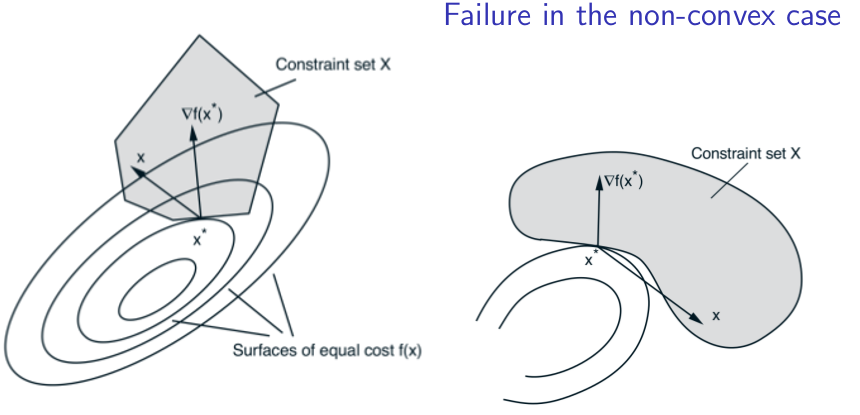
\includegraphics[width=0.8\textwidth]{non_convex}
  \caption{Illustration of the neccessary condition for constraint local minima and when it
    fails.\label{fig:non-convex}}
\end{figure}


\summary{Projection on a Convex Set}\label{s:projection-operator}

This operation is a subproblem of many constraint optimization algorithms.  Let \(z \in \RR^n\), and
\(X\) be closed and convex.  We call
\begin{equation*}
  \proj_X(z) = \min_x \enVert{x - z}
  = \min_{x}\, \frac{1}{2}\enVert{x - z}^2 \quad\text{s.t. } x \in X
\end{equation*}
the \emph{(orthogonal) projection} of \(z\) onto X (which is a different thing than the one in
Summary~\ref{s:q-conjugacy}!).  It is the point in \(X\) which is closest to \(z\).  The projection
operator for a convex set is a strongly convex function, and therefore has a unique solution.


\summary{Projection Theorem}\label{s:projection-theorem}

Given some \(z \in \RR^n\), a vector \(x^* = \proj_X(z)\) if and only if
\begin{equation*}
  \T{(z - x^*)}(x - x^*) \leq 0, \quad\forall x \in X,
\end{equation*}
since \(f(x) = \frac{1}{2} \enVert{x - z}^2\), we have \(\nabla f(x) = x - z\).  By the (neccessary
and sufficient) optimality condition we get that
\begin{alignat*}{2}
  &\quad & \T{\nabla f(x^*)}(x - x^*) &\geq 0 \\
  &\Leftrightarrow\quad & \T{(x - z)}(x - x^*) &\geq 0 \\
  &\Leftrightarrow\quad & \T{(z - x)}(x - x^*) &\leq 0.
\end{alignat*}

If \(X\) is a linear subspace of \(\RR^n\), this reduces to 
\begin{equation*}
  \T{(z - x^*)}x = 0, \quad\forall x \in X,
\end{equation*}
since for all \(x \in X\), both \(x^* + x\) and \(x^* - x\)
are in \(X\).


\summary{Quadratic Programming with Equality
  Constraints}\label{s:equality-constrained-quadratic-problems}
% bertsekas 202

We first consider the simpler problem
\begin{equation*}
  \min_x f(x) = \frac{1}{2} \enVert{x}^2 + \T{c}x, \quad\text{s.t. } Ax = 0.
\end{equation*}
By adding the constant \(\frac{1}{2} \enVert{c}^2\) to \(f\), which doesn't change the minimum, we
can write this in the equivalent form
\begin{equation*}
  \min_x \frac{1}{2} \enVert{x + c}^2, \quad\text{s.t. } Ax = 0,
\end{equation*}
which is in turn equivalent to \(\proj_X (-c)\) onto th e linear space \(X = \{x \mid Ax = 0\}\).  By
the above theorem, we therefore have the optimality condition
\begin{equation*}
  \T{(c + x^*)}x = 0, \quad\text{s.t. } Ax = 0.
\end{equation*}
Using the Lagrangian ansatz \(x^* = -c + \T{A}\mu\), we get
\begin{alignat*}{2}
  &\quad & Ax^* &= 0 \\
  &\Rightarrow\quad & - Ac + A\T{A}\mu &= 0 \\
  &\Rightarrow\quad & (A\T{A})^{-1}Ac &= \mu.
\end{alignat*}
Inserting \(\mu\) back, this gives the result
\begin{equation*}
  x^* = -c + \T{A}(A\T{A})^{-1}Ac = -(I + \T{A}(A\T{A})^{-1}A)c.
\end{equation*}

Now to the general quadratic problem
\begin{equation*}
  \min_x f(x) = \frac{1}{2} \T{(x - \bar{x})} H (x - \bar{x}) + \T{c}x, \quad\text{s.t. } Ax = b,
\end{equation*}
where \(H\) is positive definite and symmetric, and \(\bar{x}\) is an interior point
(\(A\bar{x} = b\)).  Performing a change of variables
\begin{equation*}
  y = \Sqrt{H}(x - \bar{x}) \quad\Leftrightarrow\quad x = \bar{x} + H^{-\frac{1}{2}}y
\end{equation*}
(where \(\Sqrt{H}\) and \(H^{-\frac{1}{2}}\) exist because of the assumptions), we get
\begin{align*}
  &\quad \frac{1}{2} \T{\big( \bar{x} + H^{-\frac{1}{2}} - \bar{x} \big)} H
  \big( \bar{x} + H^{-\frac{1}{2}} - \bar{x} \big) + \T{c}(\bar{x} + H^{-\frac{1}{2}} - \bar{x})
  \\
  &= \frac{1}{2} \T{\big(H^{-\frac{1}{2}}y\big)} H \big(H^{-\frac{1}{2}}y\big) +
    \T{c}H^{-\frac{1}{2}} \\
  &= \frac{1}{2} \enVert{y}^2 + \T{(H^{-\frac{1}{2}}c)}y, \qquad\text{s.t. } AH^{-\frac{1}{2}}y = 0,
\end{align*}
which can be solved by the restricted problem stated above, resulting in
\begin{equation*}
  y^* = -(I - H^{-\frac{1}{2}}\T{A} (AH^{-1}\T{A})^{-1} A H^{-\frac{1}{2}}) H^{-\frac{1}{2}}c.
\end{equation*}
Substituting back gives the optimal solution
\begin{equation*}
  x^* = \bar{x} - H^{-1}(c - \T{A}\lambda),
\end{equation*}
where
\begin{equation*}
  \lambda = (AH^{-1}\T{A})^{-1} A H^{-1}c.
\end{equation*}

\summary{Feasible Direction Methods}\label{s:feasible-direction-methods}

Given a vector \(x\), a \emph{feasible direction} at \(x\) is a vector \(d\) such that
\(x + \alpha d\) is feasible for all sufficiently small \(\alpha > 0\) (see
Figure~\ref{fig:feasible-directions}).

\begin{figure}[H]
  \centering
  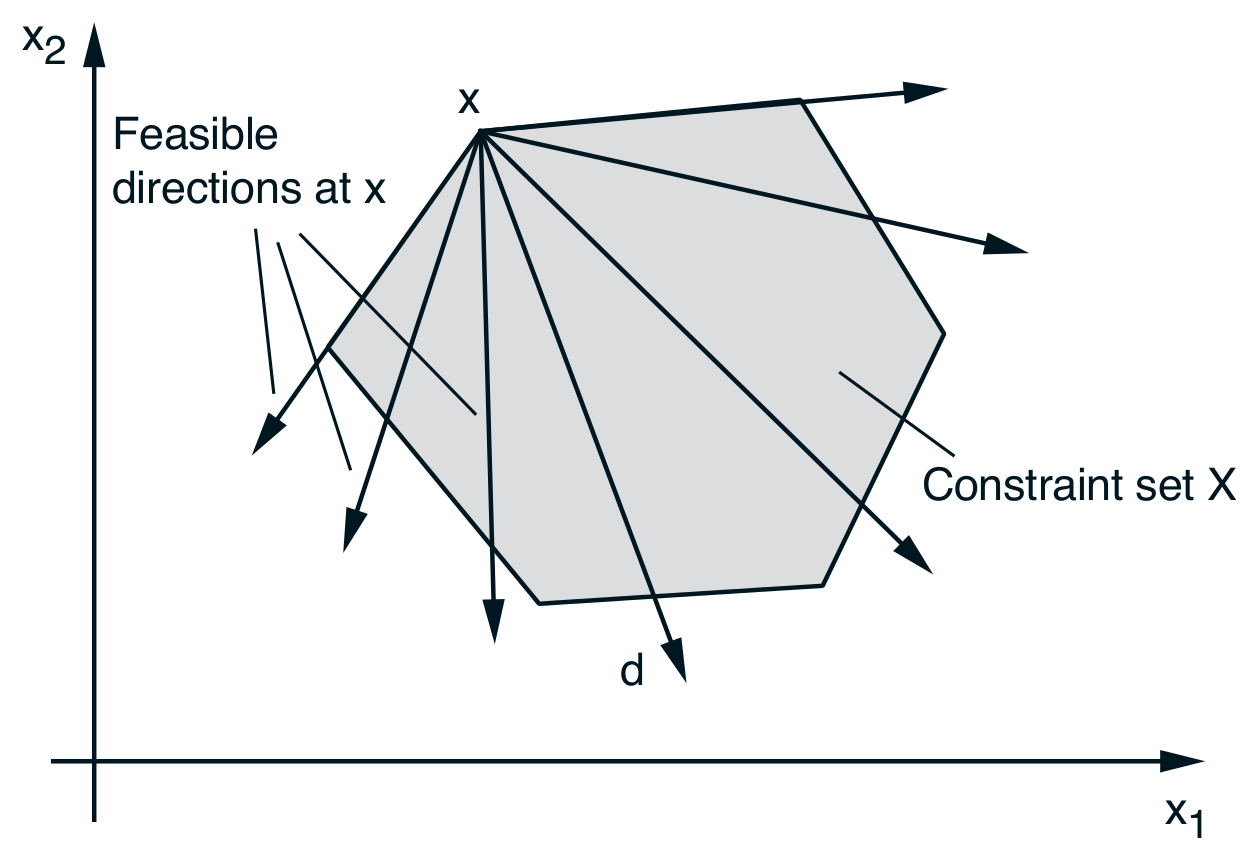
\includegraphics[width=0.5\textwidth]{feasible_directions}
  \caption{Illustration of feasible directions at \(x\) for a convex constraint
    set.\label{fig:feasible-directions}}
\end{figure}

A \emph{feasible direction method} starts with a feasible vector, and generates a sequence of
feasible points \(\{\kth{x}\}\) by
\begin{equation*}
  \kth[k+1]{x} = \kth{x} + \kth{\alpha}\kth{d},
\end{equation*}
where \(\kth{d}\) are feasible directions at \(\kth{x}\) which are also descent directions, ie.,
\begin{equation*}
  \T{\nabla f(\kth{x})}\kth{d} < 0.
\end{equation*}
The \(\kth{\alpha}\) are the step sizes satisfying \(\kth{x} + \kth{\alpha} \kth{d} \in X\).
Alternatively, since \(X\) is assumed to be convex, the feasible directions at \(\kth{x}\) can be
written in the form
\begin{equation*}
  \kth{d} = \gamma(\kth{\bar{x}} - \kth{x}), \quad \gamma > 0,
\end{equation*}
where \(\kth{\bar{x}}\) is some feasible vector different from \(\kth{x}\).  Assuming that
\(\kth{x} + \kth{\alpha} \kth{d} \in X\), the steps can be expressed as
\begin{equation*}
  \kth[k+1]{x} = \kth{x} + \kth{\alpha}(\kth{\bar{x}} - \kth{x}),
\end{equation*}
with \(\kth{\alpha} \in (0, 1]\), \(\kth{\bar{x}} \in X\), and
\(\T{\nabla f(\kth{x})}(\kth{\bar{x}} - \kth{x}) < 0\).  Since \(X\) is convex, we always have
\begin{equation*}
\kth{x} + \kth{\alpha}(\kth{\bar{x}} - \kth{x}) \in X  
\end{equation*}
for \(\kth{\alpha} \in (0, 1]\), and the sequence \(\{\kth{x}\}\) stays feasible.  Feasible
direction methods are usually presented in this form, by giving specific choices for
\(\kth{\bar{x}}\).

\summary{Step Size Selection}\label{s:step-size-selection-constrained}

Most of the rules for unconstrained optimization can be adapted for use in the constrained case
(cf. Summary~\ref{s:step-size-selection}):
\begin{itemize}
\item Limited minimization rule: \(\kth{\alpha}\) is chosen such that
  \begin{equation*}
    f(\kth{x} + \kth{\alpha}\kth{d}) = \min_{\alpha \in (0, 1]} f(\kth{x} + \alpha\kth{d}).
  \end{equation*}
  Limiting \(\alpha\) to \((0, 1]\) is no loss of generality, since different ranges can in effect
  by chosen by redefining \(\kth{d}\). 
\item Armijo rule: we fix scalars \(0 < \beta < 1\), and \(0 < \sigma < 1\), and set
  \(\kth{\alpha} = \beta^{m_k}\), where we choose \(m_k\) as the first nonnegative integer for which
  \begin{equation*}
    f(\kth{x} + \beta^{m_k} \kth{d}) - f(\kth{x}) \leq \sigma \beta^{m_k} \nabla \T{f(\kth{x})} \kth{d}.
  \end{equation*}
  (cf. Summary~\ref{s:armijo-rule})
\item Fixed step size rule: set \(\kth{\alpha}\) to a constant, e.g. \(\kth{\alpha} = 1\).
\end{itemize}

\summary{Conditional Gradient Method}\label{s:conditional-gradient-method}

A straightforward method for generating the point \(\kth{\bar{x}}\) is to find the feasible point
furthest away from \(\kth{x}\) ``along'' the negative gradient direction (see
Figure~\ref{fig:conditional-gradient-method}).  This is achieved by minimizing the directional
derivative (i.e., maximizing the descent) over the constraint set:
\begin{align*}
  \kth{\bar{x}} &\in \argmin_{x \in X} \T{\nabla f(\kth{x})}(x - \kth{x}), \\
  \kth[k+1]{x} &= \kth{x} + \kth{\alpha}(\kth{\bar{x}} - \kth{x}).
\end{align*}
Finding \(\kth{\bar{x}}\) is then a linear subproblem over a convex set, which should be easier to
solve (especially in the case that \(X\) is a simplex).  This method is also known as
\emph{Frank-Wolfe method}.

\begin{figure}[H]
  \centering
  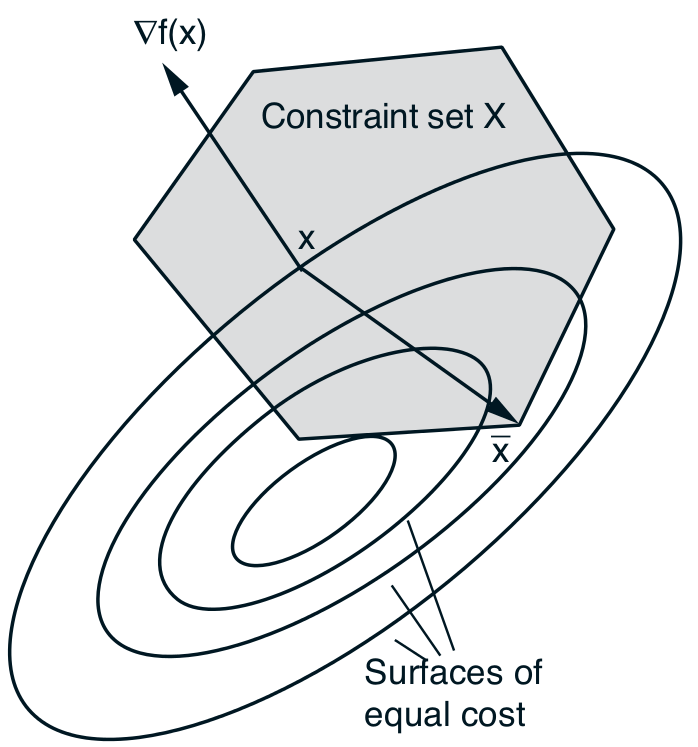
\includegraphics[width=0.3\textwidth]{conditional_gradient_method}
  \caption{Illustration of finding the feasible direction in at point \(x\) in the conditional
    gradient method. \(\bar{x}\) is the furthest point in \(X\) that lies in a descent
    direction.\label{fig:conditional-gradient-method}}
\end{figure}

\summary{Gradient Projection Method}\label{s:gradient-projection-method}

This method generates a feasible direction method with
\begin{align*}
  \kth{\bar{x}} &= \proj_X (\kth{x} - \kth{s} \nabla f(\kth{x})), \\
  \kth[k+1]{x} &= \kth{x} + \kth{\alpha}(\kth{\bar{x}} - \kth{x}),
\end{align*}
for a step size \(\kth{\alpha} \in (0, 1]\) and positive scalars \(\kth{s}\).  Thus, we take a step
in the negative gradient direction (as in steepest descent), which is then projected onto \(X\), to
obtain the feasible vector \(\kth{\bar{x}}\); see Figure~\ref{fig:gradient-projection-method}.  In
the case \(\kth{\alpha} = 1\), the method takes the easier form
\begin{equation*}
  \kth[k+1]{x} = \proj_X (\kth{x} - \kth{s} \nabla f(\kth{x})).
\end{equation*}
If \(\kth{x} - \kth{s} \nabla f(\kth{x}) \in X\), the projection is trivial and the method reduces
to steepest descent.

\begin{figure}[H]
  \centering
  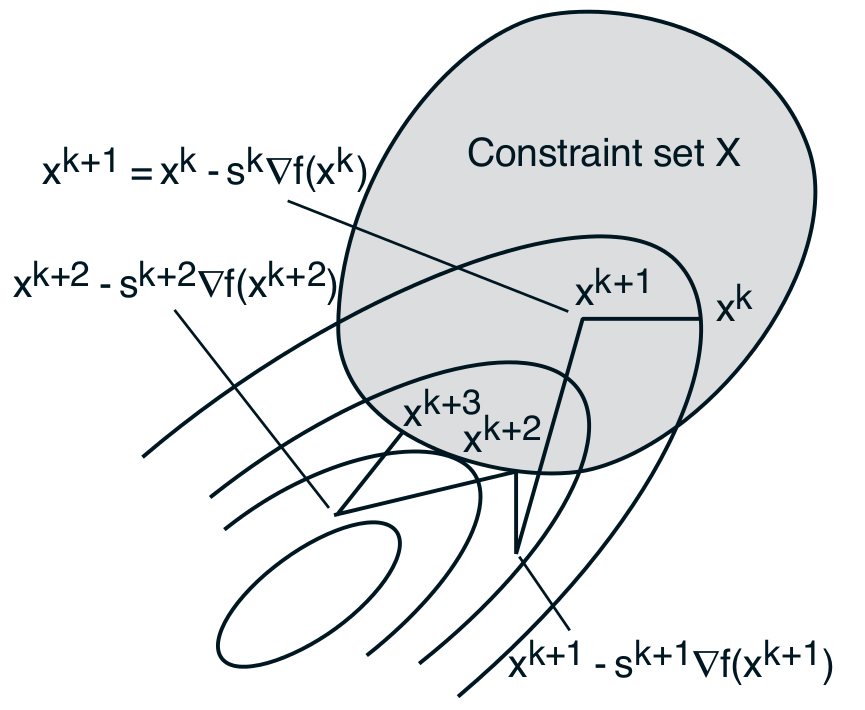
\includegraphics[width=0.4\textwidth]{gradient_projection_method}
  \caption{Illustration of the gradient projection method for \(\kth{\alpha} = 1\).  Inside \(X\),
    projection is trivial and we only do a normal gradient
    step.\label{fig:gradient-projection-method}}
\end{figure}

This method needs to solve a quadratic subproblem, which may be more complex, but typically results
in better convergence rate.

We can generalize this approach to a scaled variant, just as in steepest descent; scaling may
improve the situation with ill-conditioned objective functions, where the pure method might become
slow.  To scale, we use
\begin{equation*}
  \kth{\bar{x}} = \argmin_{x \in X} \T{\nabla f(\kth{x})} (x - \kth{x}) +
  \frac{1}{\kth{s}} \T{(x - \kth{x})} \kth{H} (x - \kth{x}).
\end{equation*}
Note that with \(\kth{s} = 1\) and \(\kth{H} = \nabla^2 f(\kth{x})\), the above expression
corresponds to a second-order expansion around \(\kth{x}\); if \(\kth{\alpha} = 1\), then
\(\kth{\bar{x}}\) just minimizes the Taylor expansion around \(\kth{x}\) in the set \(X\).  The main
disadvantage of this variant is that the subproblem might be more complicated to solve.



\summary{Linear Programming \& Affine Scaling Method}\label{s:affine-scaling-method}

% see https://ocw.mit.edu/courses/sloan-school-of-management/15-093j-optimization-methods-fall-2009/lecture-notes/MIT15_093J_F09_lec21.pdf

The affine scaling method is a specialization of the above result for linear programs with equality
constraints.  For the general problem
\begin{equation*}
  \min \T{c} x, \quad\text{s.t. } Ax = b, \; x \geq 0,
\end{equation*}
we can use the scaled projected gradient method as described above:
\begin{equation*}
  \kth[k+1]{x} = \kth{x} + \kth{\alpha}(\kth{\bar{x}} - \kth{x}),
\end{equation*}
where we have a quadratic intermediate problem
\begin{gather*}
  \kth{\bar{x}} = \argmin_x \T{c}(x - \kth{x})
  + \frac{1}{\kth{s}} \T{(x - \kth{x})} \kth{H} (x - \kth{x}),\\
  \text{s.t. } Ax = b, \; x \geq 0
\end{gather*}
for some positive definite matrices \(\kth{H}\) and positive scalars \(\kth{s}\).

Since \(\kth{x} > 0\), if \(\kth{s}\) is small enough, \(\kth{\bar{x}} > 0\), and we can drop the
inequality constraint \(x \geq 0\).  Then by the above derivation of quadratic problems
(Summary~\ref{s:equality-constrained-quadratic-problems}), we can derive the exact solution
\begin{equation*}
  \bar{x} = -\kth{x} - \kth{s}(\kth{H})^{-1}(I - \T{A} (A(\kth{H})^{-1}\T{A})^{-1} A (\kth{H})^{-1})c.
\end{equation*}
Inserting this into the iteration scheme and including \(\kth{s}\) into \(\kth{\alpha}\), we get
\begin{equation*}
  \kth[k+1]{x} = -\kth{x} -
  \kth{\alpha}(\kth{H})^{-1}(I - \T{A} (A(\kth{H})^{-1}\T{A})^{-1} A (\kth{H})^{-1})c.
\end{equation*}
Now \(\kth{\alpha}\) has to be chosen such that \(\kth[k+1]{x} > 0\).  This can be done by using
e.g. \(\kth{\alpha} = 0.99\kth{\bar{\alpha}}\), where \(\kth{\bar{\alpha}}\) is the largest step
size for which \(\kth[k+1]{x} \geq 0\) (i.e., it is still feasible).  Furthermore, \(\kth[0]{x}\)
needs to be (strictly) feasible.

Lastly, and this is the interesting part, we have to choose \(\kth{H}\).  The affine scaling method
sets it to be
\begin{equation*}
  \kth{H} = \left( \diag(\kth{x}_1, \dots, \kth{x}_n) \right)^{-2}.
\end{equation*}


\summary{Linear Programming with Inequality
  Constraints}\label{s:inequality-constrained-linear-programming}

Linear problems with inequality constraints, in the general form of
\begin{equation*}
  \max_y \T{b}y, \quad\text{s.t. } \T{A}y \leq c,
\end{equation*}
can be transformed to their dual problem
\begin{equation*}
  \min_x \T{w} x, \quad\text{s.t. } x = c - \T{A}y, \; x \geq 0
\end{equation*}
by using \(x = c - \T{A}y\) and choosing \(w\) such that \(Aw = b\).

This problem has the previous form, and thus can be solved by the affine scaling method, but we can
also write the resulting iteration form purely in terms of \(y\):
\begin{equation*}
  \kth[k+1]{y} = \kth{y} + \kth{\alpha}(A \kth{X} \T{A})^{-1} b,
\end{equation*}
with \(\kth{X} = \diag(\kth{x}_1, \dots, \kth{x}_n)\), and the step size \(\kth{\alpha}\) chosen
such that
\begin{equation*}
  \kth[k+1]{x} = c - \T{A}\kth[k+1]{y} > 0.
\end{equation*}
This variant is known as \emph{dual affine scaling method}.

%%%%%%%%%%%%%%%%%%%%%%%%%%%%%%%%%%%%%%%%%%%%%%%%%%%%%%%%%%%%%%%%%%
\section{Lagrange Multiplier Theory}

\summary{Lagrange Theorem for Equality Constrained Problems}
\label{s:lagrange-equality}

We consider the general equality constrained optimization problem
\begin{equation*}
  \min_x f(x), \quad\text{s.t. } h_i(x) = 0, \; i = 1, \dots, m,
\end{equation*}
where \(f\) and all \(h_i\) are continuously differentiable (at least in an environment around a
local minimum).  The constraints can also be compactly combined as \(h(x) = 0\).

For such a problem, the \emph{Lagrange multiplier theorem} holds: let \(x^*\) be a local minimum,
and assume that \(\nabla h_1(x^*), \dots, \nabla h_i(x^*)\) are linearly independent.  Then there
exist unique scalars \(\lambda^*_1, \dots, \lambda^*_m\), called \emph{Lagrange multipliers}, such
that
\begin{equation*}
  \nabla f(x^*) + \sum_{i=1}^m \lambda^*_i \nabla h_i(x^*) = 0.
\end{equation*}

This can be interpreted as \(\nabla f(x^*)\) being not linearly indepentent of the
\(\nabla h_i(x^*)\), i.e., at the optimal value, the gradient of the cost function belongs to the
subspace spanned by the gradients of the constraint functions.

Also, \(\nabla f(x^*)\) is orthogonal to the space of \emph{feasible variations} at \(x^*\):
\begin{equation*}
  V(x^*) = \{d \mid \T{\nabla h_i(x^*)} d = 0, i = 1, \dots, m\},
\end{equation*}
which is the the set of directions \(d\) such that \(h(x^* + d) = 0\) (i.e., the constraint is still
fulfilled).  A feasible vector for which the constraint gradients are linearly independent is called
\emph{regular}.  There may not exist Lagrange multipliers for local minima which are not regular~--
see Figure~\ref{fig:lagrange}.

\begin{figure}[H]
  \centering
  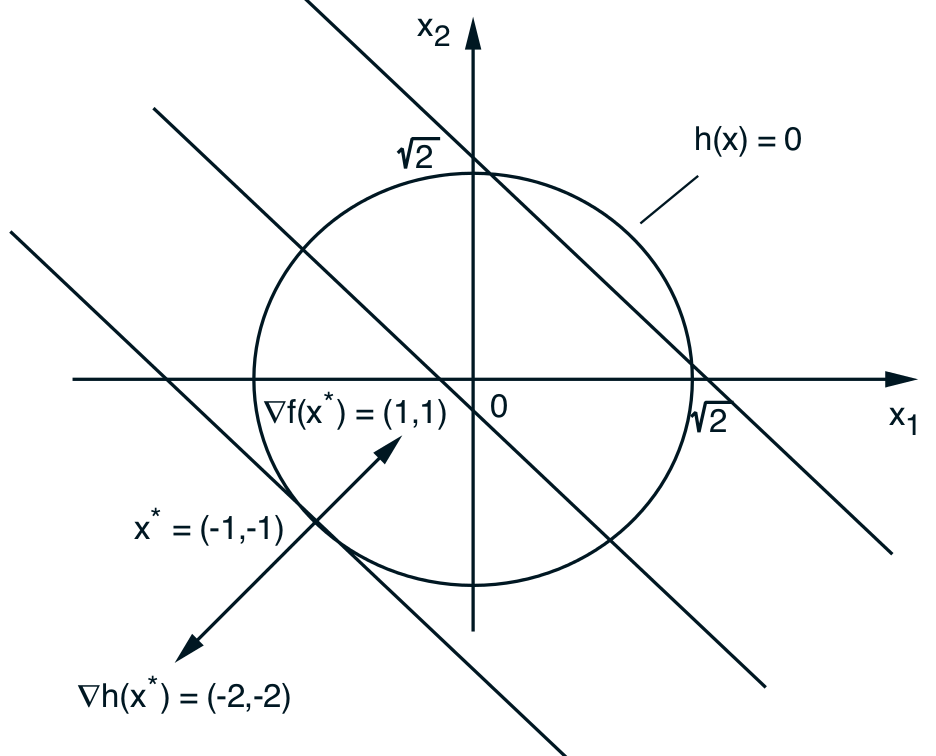
\includegraphics[width=0.45\textwidth]{lagrange_regular}
  \hspace{1em}
  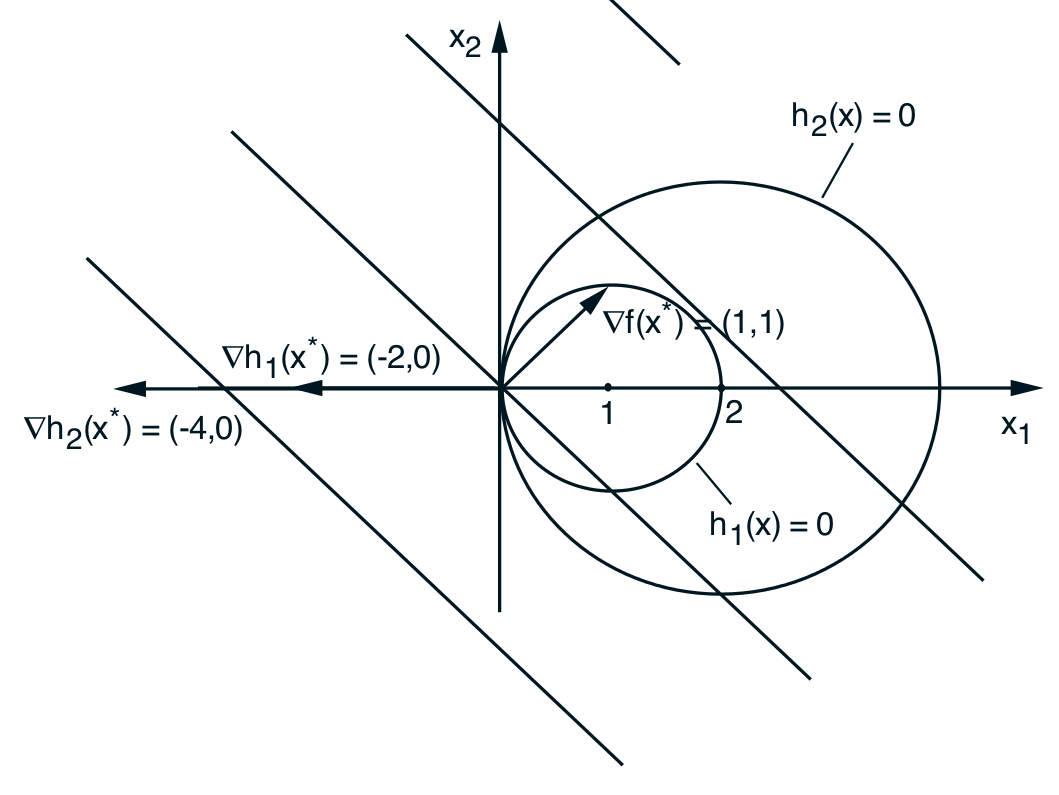
\includegraphics[width=0.45\textwidth]{lagrange_irregular}
  \caption{Left: illustration of Lagrange theorem for \(f(x) = x_1 + x_2\) subject to
    \(h(x) = x_1^2 + x_2^2 = 0\).  Right: failure in the non-regular case for
    \(h_1(x) = (x_1 - 1)^2 + x_2^2 - 1 = 0\), \(h_2(x) = (x_1 - 2)^2 + x_2^2 - 4 = 0\), where the
    constraint gradients at \(x^*\) are collinear.\label{fig:lagrange}}
\end{figure}


% \summary{Derviation of Lagrange Theorem (Penalty Approach)}
% \label{s:lagrange-derivation}

% % bertsekas 281

% The Lagrange multiplier theorem can be proven by using a penalized unconstrained cost function as
% approximation: let
% \begin{equation*}
%   \kth{F}(x) = f(x) + \frac{k}{2} \enVert[0]{h(x)}^2 + \frac{\alpha}{2} \enVert{x - x^*}^2,
% \end{equation*}
% where \(x^*\) is a local optimum and \(\alpha > 0\).  The second term imposes a penalty for
% violating the constraint, while the third one has proof-technical reasons (it constrains the value
% of \(x^*\)).

% We then select the sphere
% \begin{equation*}
%   S = \{x \mid \enVert{x - x^*} \leq \epsilon\}
% \end{equation*}
% such that \(f(x^*) \leq f(x)\) for all feasible \(x \in S\) (i.e., an environment around a local
% miniumum).  Since \(S\) is closed and bounded, there exists an optimal value \(\kth{x}\) of
% \(\kth{F}\) over \(S\) (by the Weierstrass extreme value theorem).  Now
% \begin{equation*}
%   \kth{F}(\kth{x}) = f(\kth{x}) + \frac{k}{2} \enVert[0]{h(\kth{x})}^2 +
%   \frac{\alpha}{2} \enVert{\kth{x} - x^*}^2 \leq \kth{F}(x^*) = f(x^*).
% \end{equation*}
% Since \(f\) is bounded over \(S\),
% \begin{equation*}
%   \lim_{k \to \infty} \enVert{h(\kth{x})} = 0;
% \end{equation*}
% otherwise, 


\summary{Lagrangian Function}\label{s:lagrangian-function}

Often we rewrite the constrained optimization problem in terms of a \emph{Lagrangian function}:
\begin{equation*}
  L(x, \lambda) = f(x) + \sum_i \lambda_i h_i(x).
\end{equation*}
The first order neccessary conditions for an optimum \(x^*\) are then
\begin{equation*}
  \nabla_x L(x^*, \lambda^*) = 0, \quad \nabla_\lambda L(x^*, \lambda^*) = 0.
\end{equation*}
These represent a system of \(n + m\) equations in the coordinates of \(x^*\) and \(\lambda^*\).
Every local minimum which is regular, together with the associated Lagrange vector, will be a
solution of it; however, without further assumptions, a solution need not be a minimum (it can be
any stationary point).

We furthermore have the neccesary second order condition
\begin{equation*}
  \T{d} \nabla^2_{xx} L(x^*, \lambda^*) d \geq 0, \quad\forall d \in V(x^*).
\end{equation*}


\summary{Inequality Constrained Problems}\label{s:lagrange-inequality}

We can also consider a problem involving both equality and inequality constraints:
\begin{align*}
  \min_x \quad &f(x), \\
  \text{s.t.} \quad &h_1(x) = 0, \dots, h_m(x) = 0, \\
               &g_1(x) \leq 0, \dots, g_r(x) \leq 0,
\end{align*}
where again we assume \(f\), \(h_i\), and \(g_j\) to be continuously differentiable.  We compactify
the constraints into functions \(h\) and \(g\).

To reduce the inequality constrained problem (ICP) to a form which can be treated by the above
methods for equality constrained problems (ECP), we introduce the set of \emph{active inequality
  constraints}:
\begin{equation*}
  A(x) = \{j \mid g_j(x) = 0\}.
\end{equation*}
If \(j \notin A(x)\), then the \(j\)-th constraint is said to be \emph{inactive} at \(x\).  Now, if
\(x^*\) is a local minimum of the ICP, then \(x^*\) is also a local minimum of the problem without
the inactive constrints at \(x^*\).  On the other hand, active inequality constraints can often be
treated as equalities: a local optimum of an ICP is also a local optimum for the ECP of the form
\begin{align*}
  \min_x \quad &f(x), \\
  \text{s.t.} \quad &h_1(x) = 0, \dots, h_m(x) = 0, \\
               &g_j(x) = 0, \quad\forall j \in A(x^*).
\end{align*}
This, like above, if \(x^*\) is regular, there exist Lagrange multipliers \(\lambda^*_i\) and
\(\mu^*_j\), \(j \in A(x^*)\), such that
\begin{equation*}
  \nabla f(x^*) + \sum_i \lambda^*_i \nabla h_i(x^*) + \sum_{j \in A(x^*)} \mu^*_j \nabla g_j(x^*) = 0.
\end{equation*}
Equivalently, we can write this in the form
\begin{gather*}
  \nabla f(x^*) + \sum_i \lambda^*_i \nabla h_i(x^*) + \sum_{j} \mu^*_j \nabla g_j(x^*) = 0, \\
  \text{where } \mu^*_j = 0 \text{ for all } j \notin A(x^*).
\end{gather*}
In this form, the \(\mu^*_j\) are assigned zero for inactive constraints.  Futhermore, they are all
nonnegative, since otherwise, there would exist a point with smaller cost.

Again, we call a feasible vector \(x\) \emph{regular} if the equality constraint gradients \(\nabla
h_i(x)\) and all active inequality constraint gradients \(\nabla g_j(x)\) are linearly independent.
Thus we can construct a Lagrangian function
\begin{equation*}
  L(x, \lambda, \mu) = f(x) + \sum_i \lambda_i h_i(x) + \sum_j \mu_j g_j(x).
\end{equation*}
The optima in this case are characterized the neccessary \emph{Karush-Kuhn-Tucker conditions}: if
\(x^*\) is a local minimum and regular, then there exist unique Lagrange multipliers \(\lambda^*\)
and \(\mu^*\) such that
\begin{gather*}
  \nabla_x L(x^*, \lambda^*, \mu^*) = 0, \\
  \mu^*_j \geq 0, \quad j = 1, \dots, r, \\
  \mu^*_j = 0, \quad\forall j \notin A(x^*).
\end{gather*}




% \summary{Karush-Kuhn-Tucker Optimality Conditions}\label{s:kkt-conditions}
\end{document}
